\documentclass[9pt, letterpaper, oneside]{article}

\usepackage{fancyhdr}
\setlength{\headheight}{15.2pt}
\setlength{\headwidth}{500pt}
\pagestyle{fancyplain}

\usepackage[parfill]{parskip} 
\usepackage{graphicx}
\usepackage{amsmath}
\usepackage{amssymb}
\usepackage{epstopdf}
\usepackage{fullpage}
\usepackage{cancel}
\usepackage{subfig}
\usepackage[linktoc=section, colorlinks=true, linkcolor=blue, urlcolor=blue]{hyperref}
\usepackage{tikz}
\usetikzlibrary{arrows,%
                petri,%
                topaths}%
\usepackage{verbatim}
%\setlength{\parindent}{0pt}
%\setlength{\parskip}{1ex plus 0.5ex minus 0.2ex}
\setcounter{secnumdepth}{3}
\setcounter{tocdepth}{3}
\newcommand*\dbl{\leftrightarrow}


\title{MATH 240 - Discrete Structures}
\author{McGill University \\ Fall 2011}
\date{Last Updated: \today}
\DeclareGraphicsRule{.tif}{png}{.png}{`convert #1 `dirname #1`/`basename #1 .tif`.png}

\begin{document}
\lhead{Brought to you by WikiNotes. Like our \href{https://www.facebook.com/wikinotes.ca}{facebook page} or take a look at our website on \href{http://www.wikinotes.ca}{wikinotes.ca}
\newline\line(1,0){500}}

\maketitle
\tableofcontents
\addcontentsline{toc}{section}{Course Information}

%%% Friday September 2nd 2011

\section*{Course Information}

\begin{itemize}
\item When/Where: MWF 10:35-11:35, Stewart Bio N2/2
\item Instructor: Sergey Norin math.mcgill.ca/~snorin
\item Textbook: Discrete Mathematics, Elementary and Beyond by Lovasz, Pelikan and Vesztergombi
\item Prerequisites: 
\item Grading:
	\begin{itemize}
		\item 20 \% assignments 20 \% midterm and 60 \% final
		\item 20 \% assignments 80 \% final
		\item (best of two above)
	\end{itemize}
\end{itemize}

\section*{Introduction}
Discrete vs. Continuous structures
\begin{itemize}
	\item Objects in discrete structures are individual and separable
	\item An intuitive analogy is that discrete structures focus on individual trees in the forest whereas continuous structures care about the landscape airplane view.
	\item Discrete structure courses can be called "computer science semantics" in other universities. Mathematics for computer science.
	\item Naive examples
	\begin{itemize}
		\item Counting techniques: There are two ice cream shops. One sells 20 different flavours whereas the other offers 1000 different combinations of three flavours. Which one has the most possible combinations of three flavours?
		\item Cryptography: Two parties want to communicate securely over an insecure channel. Can they do it? Yes, using number theory. Discrete Structures are used in cryptography (what this question is about), coding theorem (compression of data) and optimization.
		\item Graph Theory: Suppose you have 6 cities and you want to connect them with roads joining the least possible number of pairs, so that every pair is connected, perhaps indirectly. In how many ways can we connect these cities using 5 roads?
	\end{itemize}
	\item Before we address these problems, we must agree upon a language to formalize them.
\end{itemize}

\section{Sets}

\subsection{Definition}
A set is a collection of distinct objects which are called the elements of the set.

Examples: We use a capital letter for sets.
\begin{itemize}
	\item $A = \{ Alice, Bob, Claire, Eve \}$
	\item $B = \{ a, e, i, o, u \} = \{ o, i, e, a, u\}$
	\item $\mathbb{N} = \{1, 2, 3, 4, 5, ...\}$ (natural numbers)
	\item $\mathbb{Z} = \{.., -2, -1, 0, 1, 2, ..\}$ (integers)
	\item $\emptyset = \{\} $ (no elements, note: $\{\emptyset \} \neq \emptyset \}$)
	\item If x is an element of A we write $x \in A$ which is read "belongs", "is an element of" or "is in" e.g. $Alice \in A, Alice \notin \mathbb{N}$
	\item We say that X is a subset of a set Y if for every $z \in X$ we have $z \in Y$ Notation: $X \subseteq Y$.
	\item $\emptyset \subseteq \{1,2,3,4,5\} \subseteq \mathbb{N} \subseteq \mathbb{Z} \subseteq \mathbb{Q} \subseteq \mathbb{R} $
\end{itemize}

\subsection{Operations on sets}

$U = \{1,2,3,4,5,6 .. 10\} = \{ x \in \mathbb{N}: x \leq 10\}$

$A = \{2,4,6,8,10\} = \{x \in U: x $ is even$ \}$

$B = \{2,3,5,7\} = \{x \in U: x $ is prime$ \}$

An intersection $A \cap B$ is a set of all elements belonging to both A or B: $A \cap B = \{2\}$

A union $A \cup B$ is a set of all elements belonging to either A or B: $A \cap B = \{2,3,4,5,6,7,8,10\}$

$|A| = 5, |B| = 4, |A \cap B| = 1, |A \cup B| = 8 |\emptyset| = 0, |\mathbb{N}| = \infty$

$A - B$: all elements of A which do not belong to B $\{x : x \in A, x \notin B\}$

$A \oplus B, A \triangle B$: symmetric difference, set of all elements belonging to exactly one of A and B

\subsection{Venn Diagrams}

A way of depicting all possible relations between a collection of sets. For a set A, $|A|$ denotes the number of elements in it. 

Typically, Venn diagrams are useful for 2 or 3 sets.

\subsection{Theorems}

\begin{itemize}
	\item $A \cap (B \cup C) = (A \cap B) \cup (A \cap C)$
	\begin{itemize}
		\item Fact: For any two finites sets $|A| + |B| = |A \cap B| + |A \cup B|$
		\item Proof:
		\begin{enumerate}
			\item $x \in A \cap (B \cup C)$ then $x \in (A \cap B) \cup (A \cap C)$
			\begin{itemize}
				\item $x \in A$ and $(x \in B$ or $x \in C)$
				\item if $x \in B$ then $x \in (A \cap B)$ therefore $x \in (A \cap B) \cup (A \cap C)$
				\item if $x \in C$ then $x \in (A \cap C)$ therefore $x \in (A \cap B) \cup (A \cap C)$
			\end{itemize}
			\item $x \in (A \cap B) \cup (A \cap C)$ then $x \in A \cap (B \cup C)$
				\begin{itemize}
					\item $x \in (A \cap B)$ therefore $x \in A$ and $x \in (B \cup C)$
				\end{itemize}
		\end{enumerate}

	\end{itemize}
		\item $A \oplus B = (A \cup B)-(A \cap B) = (A - B) \cup (B - A)$
\end{itemize}

% Wednesday September 7th


\section{Logic}

Way of formally organizing knowledge studies inference rules i.e. which arguments are valid and which are fallacies.

\subsection{Propositional Calculus}

A proposition is a statement (sentence) which is either true or false.

Some examples:
\begin{itemize}
	\item $2 + 2 = 4 \to$ true
	\item $2+3 = 7 \to$ false
	\item "If it is sunny tomorrow, I will go to the beach." $\to$ valid proposition
	\item "What is going on?" $\to$ not a proposition
	\item "Stop at the red light" $\to$ not a proposition
	\item We are given 4 cards. Each card has a letter (A-Z) on one side, a number (0-9) on the other side. "If a card has a vowel on one side then it has an even number on the other" Two ways to refute this proposition: Either turn over a vowel card and find an odd number. Or turn over an odd number and find a vowel.
\end{itemize}

\subsection{Notation}
\begin{itemize}
	\item Letters will be used to denote statements: p, q, r
	\item $p \wedge q$: "and", "conjunction", "p and q" (are both true)
	\item $p \vee q$: "or", "disjunction", "either p or q" (is true)
	\item $\neg p$: "not", "p is false"	
\end{itemize}

\subsection{Truth Tables}

Making tables in \LaTeX \quad is so tedious. Check out Wesley's notes.

\subsection{Rules of Logic}

\begin{enumerate}
	\item Double negation: $\neg (\neg p) \leftrightarrow p$
	\item Indempotent rules: $p \wedge p \leftrightarrow p \qquad p \vee p \leftrightarrow p$
	\item Absorption rules: $p \wedge (p \vee q) \leftrightarrow p \qquad p \vee (p \wedge q) \leftrightarrow p$
	\item Commutative rules: $p \wedge q \leftrightarrow q \wedge p \qquad p \vee q \leftrightarrow q \vee p $
	\item Associative rules: $p \wedge (q \wedge r) \leftrightarrow (q \wedge p) \wedge r \qquad p \vee (q \vee r)\leftrightarrow (p \vee q) \vee r$
%% Friday Sept 9th 2011
	\item Distributive rules: $p \wedge (q \vee r) \leftrightarrow (p \wedge q) \vee (p \wedge r) \qquad p \vee (q \wedge r) \leftrightarrow (p \vee q) \wedge (p \vee r)$
	\item De Morgan's rule: $\neg((\neg p) \vee (\neg q)) \leftrightarrow p \wedge q \qquad \neg((\neg p) \wedge (\neg q)) \leftrightarrow p \vee q$\\
	$p \vee (\neg ((\neg p) \wedge (\neg q))) \leftrightarrow  p \vee (p \vee q) \leftrightarrow (p \vee p) \vee q \leftrightarrow p \vee q$
\end{enumerate}


\subsubsection{Conditional Statements}

\begin{enumerate}
	\item $p \to q$
	\begin{itemize}
	\item Theorem: if (an assumption holds), then (the conclusion holds).
	\item Implication: "if p then q"\\
		p = "a, b, \& c are two sides and the hypthenuse of a triangle"\\
		q = "$a^2 + b^2 = c^2$"
	\item $p \to q$ "If p then q" p implies q, p is sufficient for q\\
		$(p \to q) \leftrightarrow (q \vee (\neg p))$
		% insert truth table 1
	\item Examples: 
		\begin{itemize}
			\item "If the Riemann hypothesis is true then 2 + 2 = 4" TRUE\\
			p = "the Riemann hypothesis"\\
			q = "2+2=4"\\
			True proposition is implied by any proposition.
			\item "If pigs can fly then pigs can get sun burned" TRUE\\
			False statement implies any statement
			\item "If 2+2 =4 then pigs can fly" FALSE\\
			The implication is false only if the assumption holds and the conclusion does not.
		\end{itemize}
		% insert truth table 2
	\item $p \to q \leftrightarrow (\neg p) \to (\neg q)$
	\item $(p \to q) \wedge (q \to p) \leftrightarrow (p \leftrightarrow q)$
	\end{itemize}
\end{enumerate}

\paragraph{Puzzle}

There are three boxes A, B, C. Exactly one contains gold in it.
\begin{itemize}
	\item Box A: Gold is not in this box
	\item Box B: Gold is no in this box
	\item Box C: Gold is in box A
\end{itemize}
Exactly one of these propositions is true. Where is the gold?
Let us formalize the propositions.
\begin{itemize}
	\item p:  "Gold is in box A"
	\item q:  "Gold is in box B"
	\item r:  "Gold is in box C"
	\item Box A: $q \vee r$
	\item Box B: $p \vee r$
	\item Box C: p
	\item $p \to (p \vee r)$
	\item $\neg (p \vee r) \to q$
\end{itemize}

%%% Monday Sept 12th

\subsection{Tautologies \& Contradictions}

\paragraph{Definition}
\begin{itemize}
	\item A \textbf{tautology} is a statement that is always true (the rightmost column of the corresponding truth table has T in every row) e.g. $p \vee (\neg p)$
	\item A \textbf{contradiction} is a statement that is always false e.g. $p \wedge (\neg p)$
\end{itemize}

\paragraph{Notation}
\begin{itemize}
	\item 1 denotes a tautology
	\item 0 denotes a contradiction
	\item $1 \vee p \leftrightarrow 1$
	\item $0 \vee p \leftrightarrow p$
	\item $1 \wedge p \leftrightarrow p$
	\item $0 \wedge p \leftrightarrow 0$
\end{itemize}

\begin{itemize}
\item $p \wedge (p \vee q)$\\
\begin{tabular}{| l | l | l | l | }
  p & 1 & $p \vee q$  & $p \wedge (p \vee q)$\\
  T & T & T & T \\
  T & F & T & T \\
  F & T & T & F \\
  F & F & F & F \\
\end{tabular} \\
$\to$ Not a tautology and not a contradiction \\
$p \wedge (p \vee q) \leftrightarrow p$ (one of the rules)
\item $p \vee (p \wedge q) \vee (p \to q) \leftrightarrow (p \vee (p \wedge q)) \vee (p \to q)$ \\
$(p \to q) \leftrightarrow (\neg p) \vee q \leftrightarrow p \vee (p \to q)$\\
$\leftrightarrow p \vee ((\neg p) \vee q) (absorption)$\\
$\leftrightarrow (p \vee (\neg p))\vee q$\\
$\leftrightarrow 1 \vee q \leftrightarrow 1$
\end{itemize}

\subsection{Proofs}
\begin{itemize}
	\item $(p \to q) \wedge (q \to r) \to (p \to r)$ (always true)
	\item Implication is transitive: $p \to q \to r$
	\item A \textbf{proof} of a conclusion q given premise p is a sequence of implications (valid) $p \to p_2 \to p_3 \to .. \to p_k \to q$
	\item To prove $(p \leftrightarrow q)$ \\
		$\qquad (p \leftrightarrow q) \leftrightarrow (p \to q) \wedge (q \to p)$
	\item Theorem: Let p(x) be a polynomial then p(0) = 0 if and only if p(x) = x q(x) for some polynomial q(x)
	\item Proof: "p(0) = 0" and "p(x) = x q(x) for some polynomial q(x)"
	\begin{enumerate}
		\item $p(x) = a_nx^n + a_{n -1}x^{n-1} + ... + a_1x + a_0$ \\
			$p(0) = 0 \to a_0 = 0 \to$ \\
			$p(x) = a_nx^n + a_{n -1}x^{n-1} + ... + a_1x \to$ \\
			$p(x) = x(a_nx^{n-1} + a_{n -1}x^{n-2} + ... + a_1$ \\
			$p(x) = xq(x)$ \\
			$q(x) = a)nx^{n-1} + a_{n-1}x^{n-2} + ... + a_2$ \\
			True so proven.
		\item $p(x) = x q(x) \to p(0) = 0 \cdot q(0) \to q(0) = 0$
	\end{enumerate}
	\item Proof by contradiction: $(p \to q) \leftrightarrow ((\neg q)\to (\neg p))$
	\item Pigeonhole principle: We place an objects into m bins. If $n > m$ then some bin contains at least 2 objects.
	\item Proof: p = "$n > m$" and q = "Some bin contains at least 2 objects" \\
	$\neg q$ = "every bin contains at most 1 object" \\
	$\neg p$ = "$n \leq m$"
	$\neg q \to\ \neg p$ is trivial
	\item Theorem: There are infinitely many prime numbers \\
		Direct proof of this theorem is unlikely, there is no known simple formula producing prime numbers
	\item Proof: Assume $\neg p$. There are infinitely many prime numbers $p_1, p_2, p_3 .. p_k$ \\
	Consider $p = p_1p_2...p_k + 1$
	Every integer greater than 1 is divisible by a prime. (Prime number is the integer divisible by only 1 and itself).
	Suppose $p = p_im$ for some $1 \leq i \leq k$ and an integer m, then $p_i(p_1p_2...p_{i-1}p_{i+1}...p_k) + 1 = p_im$
	$p_i(m - p_1p_2..p_k) = 1$ (except $p_1$)
	"1 is divisible by $p_i$, a contradiction"
\end{itemize}

%%% Wednesday September 14th

\section{Circuit Complexity}

\subsection{Boolean Logic}

\begin{itemize}
	\item \textbf{Objects}: statements p, 1
	\item \textbf{Operators}: $\vee, \wedge, \neg$, etc
\end{itemize}

\subsection{Logic Gates}

Will insert logic gate diagrams later when I figure how to insert images.
%%% INSERT LOGIC GATES DIAGRAMS

\begin{tabular}{| l | l | l | l | l | }
  p & q & r  & $p \oplus q$ & $(p \oplus q) \oplus r$\\
  1 & 1 & 1 & 0 & 1 \\
  1 & 1 & 0 & 0 & 0\\
  1 & 0 & 1 & 1 & 0\\
  1 & 0 & 0 & 1 & 1\\
  0 & 1 & 1 & 0 & 0 \\
  0 & 1 & 0 & 1 & 1\\
  0 & 0 & 1 & 1 & 1\\
  0 & 0 & 0 & 0 & 0\\
\end{tabular} \\

\paragraph{Majority Circuit (for 3 inputs)}

p, q, r $\to$ 
$\begin{cases}
	$1 (or T) if at least 2 of p, q \& r are 1's$ \\
	$0 (or F) otherwise$
\end{cases}$

\paragraph{Size}
A logical circuit has size equal to the number of gates in it and depth equal to the length (or number of gates) of the longest path from an input to the final output.

Given a boolean formula, what is the minimum size (or depth) of a circuit necessary to compute it?
(depth is frequently assumed to be constant).

Given a circuit C with inputs $p_1, p_2, ..., p_n$

Can we test if C is always a contradiction? The answer is trivially yes, if we test all possible inputs. It would take $2^n$.

\subsection{Algorithms}
\begin{itemize}
	\item Every logic formula can be represented as a combinational circuit
	\item Can we represent a given formula by a "simple" circuit
	\item Given a circuit (with inputs $p_1, p_2, ..., p_n$ can we test quickly if C is a contradiction? (we can test in $2^n steps$
	\item \textbf{Algorithm}: A step-by-step procedure for solving a problem, precise enough to be carried out on a computer
\end{itemize}

%%% MISSED

%%% Friday September 16th
\section{Polytime algorithms and the P $\neq$ NP conjecture}

\subsection{Definition}
Given algorithm A its running time $t_A(n) =$ maximum number of steps the algorithm can require on inputs of size n

A is a \textbf{polynomial time} algorithm if $t_A(n)$ is polynomially bounded ($t_A(n)=O(n^2)) \dbl$ fast, efficient

P is class of problem which allow polynomial time algorithms.

\paragraph{Examples}

\begin{enumerate}
	\item Evaluating the median of a set of numbers
	\begin{itemize}
		\item Problem: $x_1, x_2, .., x_n \leftarrow$ Input
		\item Question: decide whether the median of the list is $\leq 1000$
		\item Algorithm: 
		\begin{itemize}
			\item Sort the list going once through the list ($\leq n$ steps) we can find smallest $x_i$
			\item Repeat to find the second smallest number and so on
			\item Requires $O(n^2)$ time to sort
			\item Check if $x_{\frac{n}{2}}$ is at most 1000 (roughly $n^2$ steps polytime).
		\end{itemize}
	\end{itemize}
	\item Multiplication
		\begin{itemize}
			\item Input: $2 n$ digit numbers
			\item Output: $a \times b$
			\\ roughly $n^2$ steps
		\end{itemize}
	\item Problem Factoring
		\begin{itemize}
			\item Input: a composite number C
			\item Output: Find natural numbers $a, b > 1$ such that $c = a \times b$
			\item Brute-Force search: Try all prime numbers up to c. Time: $10^{n/2} \to$ exponential time algorithm
			\item RSA ran contests until 2007 offering prizes for factoring (roughly 20 computer years for factoring 200 digit numbers)
		\end{itemize}
\end{enumerate}

\subsection{P problems}
A \textbf{polytime algorithm} is an algorithm whose running time is in order p(n) for some polynomial p.

A \textbf{decision problem} is a problem with a yes/no answer.\\
Example: 
	\begin{itemize}
	\item Input: a combinatorial circuit C (with n inputs)
	\item Output: Is C \textbf{not} a contradiction? In other words, will C output T.
	\end{itemize}

Given a decision problem D, D is in class P if there exists a polytime algorithm which solves D. It is considered to be "fast" or "efficient".

\subsection{NP problems (non-deterministic polynomial time)}

A decision problem is in the class NP if a "yes" answer always has a certificate which can be verified in polynomial time. In other words, if there is an easy way to check that the answer is yes \textbf{when} the answer is yes.

\subsubsection{The magician}

Suppose that King Arthur poses a yes/no problem to his magician Merlin. To answer such a question seems to require a tremendous amount of toil. On the other hand, if the answer to the problem is yes, there is a piece of evidence or \textbf{certificate} to quickly verify the yes-ness.

Examples
\begin{itemize}
	\item In the circuit example above, if there exists a set of values for inputs so that the circuit outputs 1 (or T) then given this collection of inputs, we can easily verify that the circuit is not contradictory. 
	\item Traveling salesman problem:
		\begin{itemize}
			\item Input: Collection of n cities where the ith city is located at $(x_i, y_i)$ and the distances between them
			\item Output: A tour such that each city is visited exactly once and the total length $\leq 1000$ miles
			\item Checking each possible tour amounts to (a) fixing some city from which to start then (b) choosing a second city (999 choices) and a third city (998 choices and so on. Thus the number of tours is $999!$. This requires a tremendous amount of computation that is way beyond polynomial time.
			\item If however, you somehow come up with a tour (use magic), you can easily test if it matches the requirements by computing the sum of distances between two adjacent cities i.e.\\ $\sqrt{(x_{1000} - x_1)^2 + (y_{1000} - y_1)^2} + \sum{\sqrt{(x_{i} - x_{i+1})^2 + (y_{i} - y_{i+1})^2}} \leq 1000$
			\item It doesn't matter if Merlin didn't heck all 999! possible tours, only that he found one that worked and that we could prove quickly that it did work
		\end{itemize}
	\item Factoring
		\begin{itemize}
			\item Input: n digit number
			\item Output: Is this number composite and if it is, factor it.
			\item If the magician comes up with a set of factors, it is easy to check if the factors are prime and easy to check if their product is the n-digit number.
		\end{itemize} 	
\end{itemize}

\subsubsection{Definition}
A decision problem D is in class NP if there is a polytime algorithm M (called the checking algorithm) and a polynomial p which given an input and some "extra information" called certificate can verify that x is indeed in L.

It is easy to see that $P \subseteq NP$ i.e. every P-class decision problem is in class NP since if A is a polytime algorithm which solves the decision problem D, then it will also suit as the checking algorithm in the definition of NP. We do not even need a certificate to prove it.

\subsection{$P \neq NP$}

There exist problems which cannot be solved efficiently but for which a positive answer can be verified efficiently. There exists problems for which brute-force search is essentially the best possible strategy. If there are problems where you need a magician, then it is NP.

If there exists a problem in NP but not in P (if the conjecture is true) then testing if a circuit is a contradiction, travelling salesman problem, and a very large class of similar problems are all not in P

If P = NP then airline scheduling, protein folding, packing boxes, finding short proof for theorems all can be done efficiently but certain cryptography becomes impossible.

The universal opinion is that $P \neq NP$

\subsubsection{Scott Aoronson's reasons for $P \neq NP$}

Empirical: Problems in NP remain heuristically hard, however problems which are now known to be in P (linear programming, primality testing) but efficient heuristics existed long before. 

(N.B. I don't know what this is supposed to mean. Here's a Scott Aoranson quote though:

If P = NP, then the world would be a profoundly different place than we usually assume it to be. There would be no special value in "creative leaps," no fundamental gap between solving a problem and recognizing the solution once it's found. Everyone who could appreciate a symphony would be Mozart; everyone who could follow a step-by-step argument would be Gauss... )
%%%%% Monday September 19th

\section{Proof Techniques: Predicate calculus}

\paragraph{Reminder}

A proof is a sequence of implications deriving a conclusion q from a premise p: $p \to q$

\begin{itemize}
\item Direct Proof: $p \to p_1 \to p_2 \to p_3 .\to ... \to p_k \to q$
\item Proof by contradiction: $p \to q \dbl (\neg q \to \neg p)$
\item Case Analysis: $(p \wedge q \to r) \dbl (p \to r) \wedge (q \to r)$ See below
\item Counter Examples: See below
\end{itemize}

\paragraph{Case Analysis}
\begin{itemize}
\item \textbf{Proposition}: For positive integer n: $3 \nmid n \to 3 \mid n^2 + 2$\\
	($a\mid b \to$ "a divides b" there exists an integer c, b = ac)\\
	\textbf{Proof}: Divide n by 3 with remainder such as $n = 3q + r \qquad q \in \mathbb{N}, 0 < r < 3$
	\begin{itemize}
		\item $r = 1 \to n = 3q + 1 \\ n^2 + 2 = 9q^2 + 1 + 6q + 2 = 3 \cdot (3q^2 + 2q + 1)$ \\ therefore divisible by 3  
		\item $r = 2 \to n = 3q + 2 \\ n^2 + 2 = 9q^2 + 4 + 12q + 2 = 3 \cdot (3q^2 + 6q + 2)$ \\ therefore divisible by 3  
	\end{itemize}
\end{itemize}

\paragraph{Counter Example}
	\begin{itemize}
		\item Proposition: $n^2 + n + 1$ is prime for every positive integer n $\leq$ 10
		\item $4^2 + 4 + 1 = 21 = 7 \cdot 3$
		\item This is a counter example: the statement is false
		\item Mathematical Notation
		\begin{itemize}
		\item $p \to q \wedge r \to p \to q$ if $\neg(p \to q) \to \neg(p \to q \wedge r)$ 
		\item q is a counter example to the implication "$n^2 + n + 1$ is prime for all integers n " 			\item "$n^2+ n + 1$ is prime" $\leftarrow$ P(n) predicate proposition depending on a variable
		$\forall n \in \mathbb{Z}(P(n))$\\
		Note: $\forall$  means "for all" e.g. "For all n in the set of integers the predicate "$n^2 + n + 1$"is prime" is true
		\item "There exists an integer n so that $n^2 + n + 1$ is not prime" is noted $\exists n \in \mathbb{Z}(Q(n))$ where Q(n) "$n^2 + n + 1$ is not prime" i.e. $Q(n) = \neg P(n)$
		\end{itemize}
\end{itemize}

\paragraph{Goldback's conjecture}
Every even integer bigger than 2 is expressible as a sum of 2 primes.
\begin{itemize}
\item $\forall n \in$ "even integers", $n > 2 \to (\exists a, b \in \{primes\} (n = a + b))$)
\item
In predicate calculus, "71 is prime" is equivalent to the notation: \\ $\forall a, b \in \mathbb{N} ( a \cdot b = 71) \to ((a = 1) \wedge (b=71))$
\end{itemize}

\paragraph{Limits}
Various ways to say the same thing:
\begin{itemize}
\item "As x approaches a, f(x) becomes closer and closer to L"
\item "f(x) has a limit L as x $\to$ a" 
\item "$lim_{x \to a} f(x) = L$"
\item "For every $\epsilon > 0$, there exists $\delta > 0$ so that if $| x - a | < \delta$ then $|f(x) - L |< \epsilon$"
\item "$\forall \epsilon > 0 \quad (\exists \delta > 0 \quad (|x-a|<\delta \to |f(x) - L | < \epsilon))$
\item "$lim_{x \to \infty} f(x) = L" \dbl \quad \forall \epsilon > 0 \quad (\exists X : \quad (\forall x > X \quad (|f(x) - L| < \epsilon)))$
\end{itemize}

\paragraph{Negation}
\begin{itemize}
\item
$\neg(\forall n \in A : P(n)) \dbl \exists n \in A \quad (\neg P(n))$
\item
$\forall n \in A : P(n) \dbl \neg(\exists n \in A \quad (\neg P(n)))$
\item
This is very useful in proofs, since proving $(\forall n \quad (p(n))$ might be hard if we consider all
values of n, whereas checking that there can't be a value of n such that p(n) does
not hold could be easier.
\end{itemize}
\paragraph{"$\sin x$ does not have a limit as $x \to \infty$"}
\begin{align*}
\neg(\exists L : lim_{x \to \infty} \sin x = L)
&\dbl \forall L : (\neg (lim(\sin x) = L)\\
&\dbl \forall L \quad (\neg(\forall \epsilon > 0 \quad (\exists X \quad (\forall x > X \quad (|\sin x - L| <\epsilon)))))\\
&\dbl \forall L \quad (\exists \epsilon > 0 \quad (\neg (\exists X  \quad (\forall x > X \quad (|\sin x - L| <\epsilon)))))\\
&\dbl \forall L \quad (\exists \epsilon > 0 \quad (\forall X \quad (\exists x > X \quad (|\sin{x} -L | \geq \epsilon))))\\
\end{align*}

%%% Wednesday September 21st

\subsection{Divisibility Problem}
We want to prove the following theorem:
\begin{itemize}
\item Any collection of n+1 numbers chosen from the set \{1,2,...,2n\} contains two numbers so that one is divisible by the other.
\item $\forall n \in \mathbb{N} \quad (\forall S \subseteq \{1,2,...,2n\} \quad ((|S| = n + 1) \to \exists a,b \in S \quad ((a | b) \wedge (a \neq b))))$
\end{itemize}

\paragraph{Reminder: the pigeonhole principle} 

If $n+1$ objects are placed into n boxes then some box contains $\geq 2$ objects. To apply the principle we want to partition $\{1,2,...,2n\}$ into n subjects. 

\paragraph{Partition} We say that a collection $A_1, A_2, ... A_k$ of subsets of a set B is a \textbf{partition} of B if
\begin{enumerate}
	\item $\forall i,j : 1 \leq i < j \leq k \qquad A_i \cap A_j = \emptyset$ (no element of B belongs to two different parts)
	\item $A_1 \cup A_2 \cup ... \cup A_k = B$
\end{enumerate}

Example: \{1,2,3,4,5,6,7,8\} can be partitioned into \{1,2,4,6,8\} , \{3, 5\} , \{7\}

\paragraph{Proof} By the pigeonhole principle it suffices to find a partition $A_1, A_2, ... A_n$ of \{1,2,...,2n\} so that\\
$(\forall i \quad (\exists a,b \in A_i \quad (a | b \vee b | a)))$

Here is a construction:
$A_i = \{(2i - 1), 2(2i -1), 4(2i -1), ..., 2^m(2i-1)\}$ up to maximum m: $2^m (2i-1) \leq 2n$
\begin{enumerate}
\item $A_i$ satisfies the desired property for all i
\item $A_1, A_2, .., A_n$ is a partition of \{1,2,...,2n\} \\
Ever positive integer can be uniquely written in a form $2^m(2i - 1)$ for some $i \geq 1, m \geq 0$
\end{enumerate}

Note: Is it true for some n:
"Every collection of n numbers chosen from \{1,2,...,2n\} contains 2 numbers one dividing the other"?

Counter-example: $n = 2 \quad \{1,2,3,4\} \to \{3,4\}$

%%% missed big chunk here


\subsection{Strangers and Clubs}

For a collection of people any two of them either have met or haven't . A club is a group of people who have pairwise met each other. A group of strangers is a group of people who pairwise have not met each other

Theorem: In any collection of 6 people there is either a club of 3 people or a group of 3 strangers.

Proof Let x be one of the people in the collection. The following cases apply
\begin{enumerate}
	\item x has at least 3 acquaintances
	\begin{enumerate}
		\item Some two of acquaintances of x, say y \& z know each other. Then \{x, y, z\} form a club.
		\item No two acquaintances of x know each other. Then they form a group of strangers.
	\end{enumerate}
	\item x has at most 2 acquaintances. There are at least 3 people that x does not know. Now the argument is in case 1 with acquaintances replaced by strangers.
\end{enumerate}

\section{Social Choice Function}

\subsection{Definition}
3 candidates A, B \& C:
\begin{itemize}
	\item 49\% of electorate $A > B > C$
	\item 48 \% of electorate $B > A > C$
	\item 3\% of electorate $C > B > A$
\end{itemize}

Given a collection of voters $v_1, v_2, ..., v_n$ and several candidates A, B, C, D, ...

Each voter ranks the candidates according to his preferences:

$A >^{v_2} B >^{v_2} C >^{v_2} D \qquad $where $>^{v_i} $ is the ordering produced by the $i^{th}$ voter

\paragraph{Permutation}

(A, D, B, C) of the set of candidates \{A, B, C, D \}

Social choice function takes as an input voter's ordering and produces a consensus ordering $f(>^{v_1},>^{v_2},,...,>^{v_n}) = \quad >$

What conditions should a good SCF satisfy?
\begin{enumerate}
	\item \textbf{Unanimity}: If every voter prefers $\alpha$ to $\beta$ then the consensus ordering must rank $\alpha$ above $\beta$ \\
	$(\forall v \quad (\alpha >^{v} \beta)) \to (\alpha > \beta)$
	\item \textbf{Independence on irrelevant alternatives (IAA)}
	The final relative ordering of $\alpha$ and $\beta$ (higher, lower or indifferent) should depend only on relative orderings of $\alpha$ and $\beta$ by every individual (If a candidate withdraws from election this doesn't affect the order of others). 
\end{enumerate}

Which social choice functions satisfy these properties?

What happens with majority? $\alpha > \beta$ if more than half of the voters prefer $\alpha$ to $\beta$:
\begin{itemize}
	\item $v_1 : A >^{v_1} B >^{v_1} C $
	\item $v_2 : C >^{v_2} A >^{v_2} B $
	\item $v_3 : B >^{v_3} C >^{v_3} A $
\end{itemize}

How does this work? There is a conflict here...

\textbf{Dictatorship}: For some fixed voter d we have ($\alpha > \beta$) if and only if ($\alpha >^d \beta$) i.e. society prefers $\alpha$ to $\beta$ whenever d strictly prefers $\alpha$ to $\beta$

\subsection{Arrow's impossibility Theorem (1951)} 
\textbf{Theorem:} Any constitution that respects independence of irrelevant alternatives and unanimity is a dictatorship.

\paragraph{Proof}

Unanimity $\wedge$ IIA $\to$ dictatorship

Let $>$ satisfy these two properties $\beta$ is called a polarizing candidate if every voter ranks him.her at the very top or the very bottom of the list.

\textbf{Claim} A polarizing candidate ranks first or last in the consensus ordering $>$

\textbf{Proof} Suppose not $\alpha > \beta > \gamma $ where $\beta$ is a polarizing candidate

\begin{tabular}{| l | l | l | l | }
  $\beta$ & $\beta$ & $\alpha$  & $\gamma$\\
  $\alpha$ & $\gamma$ & $\gamma$  & $\alpha$\\
  $\gamma$ & $\alpha$ & $\beta$  & $\beta$\\
\end{tabular}

Switch $\alpha$ and $\gamma$ in voter's preferences so that every voter prefers $\gamma$ to $\alpha$. We should still have $\alpha > \beta > \gamma$ because relative positions of $\alpha$ and $\beta$ and relative positions of $\beta$ and $\gamma$ are unchanged. By unanimity we should now have $\gamma > \alpha$ (contradiction QED)


Choose a candidate $\beta$

\begin{tabular}{| l | l | l | l | }
  $\beta$ & $\beta$ & $\alpha$  & $\gamma$\\
  $\alpha$ & $\gamma$ & $\gamma$  & $\alpha$\\
  $\beta$ & $\beta$ & $...$  & $\beta$\\
  $v_1$ & $v_2$ & $...$  & $v_n$\\
\end{tabular}
$\to$
\begin{tabular}{| l | l | l | l | }
  $\beta$ & $-$ & $-$  & $-$\\
  $\alpha$ & $\gamma$ & $\gamma$  & $\alpha$\\
  $-$ & $\beta$ & $...$  & $\beta$\\
  $v_1$ & $v_2$ & $...$  & $v_n$\\
\end{tabular}

%%% missed

So there exists a voter $v^*$ so that
\begin{tabular}{| l | l | l | l | }
  $\beta$ & $-$ & $-$  & $-$\\
  $\alpha$ & $\gamma$ & $\gamma$  & $\alpha$\\
  $-$ & $\beta$ & $...$  & $\beta$\\
  $v_1$ & $v_2$ & $...$  & $v_n$\\
\end{tabular}

Goddammit. Disregard this last section (the whole theorem). I will fix it later.

\section{Proofs}

\subsection{The well-ordering principle}
\begin{itemize}
	\item \textbf{The well-ordering principle} \\
	Every non empty subset of non-negative integers has a smallest element.
	\item \textbf{The induction principle}\\
	 "P(n) is true for all natural numbers b"
\end{itemize}

\subsubsection{Proofs using the well-ordering principle}

\paragraph{Claim}
There exists subsets of non-negative rational numbers with no smallest element.

$\{x \in \mathbb{Q} | x > 1\}$ ($\mathbb{Q}$ is the set of rational numbers\}

Suppose $x_0<x_1$, $x_0 \in \mathbb{Q}$ is a smallest element of this set $x_0 = \frac{m}{n} \quad m > n$

(missed)
%$1 < x^1 = $
\paragraph{Proving the irrationality of $\sqrt{2}$}
\begin{itemize}
	\item \textbf{Theorem} $\sqrt{2}$ is irrational.
	\item \textbf{Proof} Suppose $\sqrt{2}$ is rational (Proof by contradiction) \\
		$c = \{m \in \mathbb{N} | \exists n \in \mathbb{N} (\sqrt{2} = m / n)\}$ \\
		Our assumption is equivalent to the statement $C \neq \emptyset$ \\
		By the well-ordering principle there exists $m_0$ the smallest element of C \\
		$\sqrt{2} = \frac{m_0}{n_0} \to 2 = \frac{m_0^2}{n_0^2} \to 2n_0^2 = m_0^2 \to m_0 = 2m' \to 2n_0^2 = 4m'^2 \to n_0^2 = 2m'^2 \to n_0 = 2n' \to (2n')^2  = 2m'^2 \to 2n'^2 = m'^2 \to \sqrt{2}n' = m' \to \sqrt{2} = \frac{m'}{n'} \to m \in C$ but $m' < m_0$
	\item	There is a contradiction as $m_0$ was chosen to be the smallest element of C.
\end{itemize}

\subsubsection{Method}
Structure of the proofs using well-ordering principle: \\
"P(n) is true for all positive integeres n" (In our theorem P(m) := "$\neg(\exists n \in \mathbb{N} \quad \sqrt{2} = \frac{m}{n})$"
	\begin{enumerate}
		\item $C = \{ n \in \mathbb{N} |$ P(n) is False $\}$
		\item Assume for a contradiction that $C \neq \emptyset$
		\item By the well-ordering principle we can choose $n_0$ the smallest element of C
		\item Obtain the contradiction to this choice (for example show that $n_0 \notin C$)
	\end{enumerate}

Theorem
Every positive integer bigger than 1 can be expressed as a product of prime numbers (being prime counts).

Statement
P(n) = "If n > 1, then n can be expressed as product of prime numbers

C = $\{n \in \mathbb{N} : n > 1$ n can be expressed as such a product\}

Choose $n_0$ to be a smallest element of C (We are using proof by contradiction)

\begin{itemize}
	\item Case 1: $n_0$ is prime \\
	This can't happen. $n_0$ by itself would be a valid product
	\item Case 2: $n_0$ is not prime \\
	      $n_0 = ab \qquad 1 < a,b < n_0 \qquad a,b \in \mathbb{N}$ \\
	      Therefore as $a, b \notin C$, so $a = p_1p_2p_3...p_k \quad p_i$ is prime and 
	      						$b = q_1q_2 ... q_i \quad q_j$ is prime \\
	       $n = p_1p_2p_3...p_k . q_1q_2q_3...q_k \quad$ So n is a product of primes \\
	       $n \notin C \to$ contradiction
\end{itemize}

\paragraph{What is the sum of the first n odd (+) integers?}

1 + 3+ 5 +... + (2n-1)

\begin{align*}
1 &= 1
1 + 3 &= 4
1 + 3 + 5 &= 9
1+ 3 + 5 + 7 &= 16
\end{align*}
It looks like the answer is $n^2$ (but this is not enough to prove it)

\paragraph{Theorem:} $1 + 3 + 5 + 7 + ... + (2n-1) = n^2$

\textbf{Proof}: Suppose for a contradiction that $n_0$ is the smallest positive integer for which this formula is false

$1 + 3 + 5 + ... + 2n -1 \neq n_0$

The formula is true for $n_0 -1 \qquad (n_0 \neq 1)$

$1 + 3 + 5 + ... + 2(n_0 -1) -1 = (n_0 - 1)^2$

So $1 + 3 + 5  + ...+ (2n-1) = (n_0 -1)^2 + 2n_0 -1 = n_0^2 \to$ contradiction!

\subsection{Induction}

\paragraph{Method}
"P(n) is true for all n $\in \mathbb{N}$ if
\begin{enumerate}
	\item Base of induction: "P(1) is true"
	\item Induction steps: "P(n-1) implies P(n) for all $n \geq 2$ \\
	(Equivalently  "P(n) implies P(n+1) for all $n \geq 1$"
\end{enumerate}

\subsubsection{A few examples}

\paragraph{Sum of n first Integers}
\begin{itemize}
	\item \textbf{Theorem}: $1 + 2 + ... +n = \frac{n(n+1)}{2}$
	\item \textbf{Proof}: By induction on n
	\item \textbf{Base case n =1}: $1 = \frac{1}{1+1}/2 = 1$
	\item \textbf{Induction step:} $P(n) \to P(n+1) for n \geq 1$\\
			$1 + 2 + ... + n = \frac{n(n+1)}{2}$
			$P(n+1): 1 + 2 + ... +n + (n+1) = \frac{n(n+1)}{2} + (n + 1) = (n + 1) \cdot ( \frac{n}{2} + 1) = \frac{(n+1) \cdot (n + 2)}{2} \Box$
\end{itemize}

\paragraph{$2^n \geq n^2$}
\begin{itemize}
	\item \textbf{Theorem}: $2^n \geq n^2 \forall n \geq 4$
	\item Base case: $n = 4, 2^4 = 16 = 4^2$
	\item Induction step: $(2^n \geq n^2) \to (2^{n+1} \geq (n+1)^2)$
		\begin{align*}
		2^{n+1} &= 2^n \cdot 2 \\
		&\geq 2n^2 = n^2 + n^2 \\
		&\geq n^2 + 4n \qquad (n \geq 4) \\
		&\geq n^2 + 2n + 1 = (n + 1)^2 \qquad (2n \geq 1) \\
		\end{align*}
\end{itemize}

\paragraph{A flawed induction proof}
\begin{itemize}
	\item Theorem: All horses are the same colour
	\item Base Case: One horse is the same colour as its self
	\item Induction step: Any n horse are the same colour. Any n + 1 horses are the same colour.
\end{itemize}

Flaw: P(n) does not imply P(n+1)
%%% Write this later

\section{Number Theory}

\paragraph{Definition}
Studies properties of integers: divisibility, primes. an integer a divides an integer b if \\ ($ \exists x \in \mathbb{Z} : \quad (xa=b)$

Division with remainder: for any two integers $a > 0$ and b there exists integers q and d  so that \\ $b = qa + r \to$ r is the remainder with $0 \leq r \leq a$

We write $a | b$, if and only if $r = 0$

A positive integer $p > 1$ is prime if the only positive integers dividing p are 1 and p

An integer $n > 1$ is composite if it is not prime

Expression of a positive integer as product of primes is called prime factorization.

\paragraph{The fundamental theorem of arithmetic} Every integer greater than 1 admits unique prime factorization

\textbf{Proof using contradiction}: Suppose some n admits at least two distinct prime factorizations. Choose the minimum such n.

$n = p_1 \cdot p_2 \cdot p_3 \cdot ... \cdot p_k = q_1\cdot q_2 \cdot ...\cdot q_l$

We may assume that $p_1$ is the smallest prime among all the primes $p_i$ and $q_j$

Suppose $p_1 = q_1$ then $\displaystyle\frac{n}{p_i} = p_2 \cdot ... \cdot p_k = q_2 \cdot ... \cdot q_l$

It is a smaller number admitting two different factorizations

$p_1 < q_1$ so $q1 = xp_1 + r \qquad 0 \leq r \leq p_1$

$n = (xp_1 + r )q_2 ... q_i$ also we may assume $q_2, q_3 , ... q_l \neq p_1$

$p_1 | n$ 

$n = xp_1\cdot q_2 \cdot ... \cdot q_l + r \cdot q_2 \cdot .... \cdot q_l$

$n$ is divisible by $p_1$

$n > m > 1 \qquad m = r \cdot q_2...q_l$ is divisible by $p_1$

$m < n$ as $x > 0$ because $q_1 > p_1 > r$

We will sow that m also has two different prime factorizations 

$m = p_1m = p_1r_1r_2...r_s \to$ there exists a prime factorization of m which includes 

A contradiction to the choice of..

(missed)
% missed


%%% Friday September 30th 2011

\subsection{Primes}

\paragraph{Fundamental theorem of arithmetic} Every integer greater than 1 can be uniquely expressed as a product of primes

$a=p_1^{r1}p_2^{r_2}...p_k^{r_k}$
$b = p_1^{s_1}p_2^{s_2}...p_k^{s_k}$

$1200 = 2^4\cdot 3 \cdot 5^2$

$[ab = p_1^{r_1 + s_1} p_2^{r_2 + s_2} ... p_k^{r_k + s_k}]$

$a | b$ if and only if $r_i \leq s_i$ for all $1 \leq i \leq k$

\begin{itemize}
    \item \textbf{Theorem} $\sqrt{2}$ is irrational
    \item \textbf{Proof}: Suppose $\sqrt{2}$ is not \\
    then $\sqrt{2} = \frac{m}{n} = 2 = \frac{m^2}{n^2}$ \\
    ($m = 2^r p_1^{r_1} \ldots p_k^{r_k}$)\\
    ($n = 2^s p_1^{s_1} \ldots p_k^{s_k}$)\\
    $(2n^2 = m^2$)\\
    ($2n^2 = 2^{2s+1} p_1^{2s_1} \ldots p_k^{2s_k}$)\\
    ($m^2 = 2^{2r} p_1^{2r_1} \ldots p_k^{2r_k}$)\\
    Contradiction as ($2s+1 \neq 2r$)
    \item \textbf{Theorem:} $\sqrt{n}$ is rational for any integer n if and only if $n = k^2$ for some k
\end{itemize}

Proof: Exercise. Modify the proof for $\sqrt{2}$

\begin{itemize}
    \item \textbf{Theorem}: If a prime $p | ab$ then either $p | a$ or $p| b$
    \item \textbf{Proof}: if p is not present in the prime factorization of either a or b, then it is not present in the prime factorization of $a \cdot b $ and so $p \nmid a b$
    \item Is this true when p is not prime? Suppose we have $p_1 \cdot p_2$ instead of $p_1$ then $p_1 | a$ or $p_1 | b \qquad$ $p_2 | 1$ or $p_2 | b$
\end{itemize}

--------------

$2,3,5,7,11,13,17,19,23,29,31,37,41,43$
\begin{enumerate}
    \item There are infinitely many prime numbers.
    \item Prime numbers are not everywhere dense in natural numbers. There are large gaps
\end{enumerate}

\begin{itemize}
    \item \textbf{Theorem} For any positive integer k there exists two consecutive prime numbers with difference $\geq k$
    \item \textbf{Proof} It suffices to exhibit a sequence of $\geq k$ consecutive composite numbers\\
            $n! = 1 \cdot 2 \cdot 3 \cdot 4 \cdot ... \cdot (n-1) \cdot n$\\
            Let $n = k + 1$\\
            $n! + 2, n! + 3, n! + 4, n! + 5,..., n! + n \to k$ consecutive integers all composite\\
            $n! + m$ is composite for all $2 \leq m \leq n \qquad m | n! + m \leftarrow m| n! \qquad 2 \leq m \leq n! + m$
    \item \textbf{Twin prime conjecture} There exist infinitely many pairs $p, p+2$ so that they are both primes. (This question has been asked more than 2000 years ago.)
    \item \textbf{The prime number theorem:} For a number n let $\pi(n)$ denote the number of primes $\leq n$. Then \\
            $\pi(n) \cong \frac{n}{\ln n} \qquad lim_{n \to \infty} \frac{\pi(n)}{n / \ln n} = 1$ \\
            Average gaps between primes are $\cong \ln n$ 
    \item \textbf{Conjecture} For every positive integer n there exists a prime p $n^2 \leq p \leq (n+1)^2$
    \begin{enumerate}
        \item It is possible to efficiently test whether a number is prime or composite.
        \item It is believed not to be possible to efficiently produce prime factorisations.
    \end{enumerate}
\end{itemize}

\subsection{Greatest common divisors and linear combinations}

\paragraph{Die Hard 3 Problem} A jug containing precisely 4 gallons of water deactivates the bomb. He has a 3 gallon, a 5 gallon jug and 5 minutes. Given an a-gallon jug and a b-gallon jug, what ammounts can we get?

$a \leq b$ let (x,y) record current amounts of water in jugs of size a and b respectively

Here is an example of our approach
\begin{enumerate}
    \item (a,0) - fill in the first jug
    \item (0,a) - pour first jug into the second
    \item (a,a) - fill in the first one again
    \item (2a-b, b) - pour first into second
    \item (2a-b, 0) - empty the second jug
    \item (0, 2a-b)
    \item (a, 2a-b)
    \item (0, 3a-b) $\to$ John Mclane survives $3 \cdot 3 - 5 = 4!$
\end{enumerate}

\subsection{Linear Combinations}
\begin{itemize}
    \item A linear combination of a and b is an integer expressible as $sa + tb$ where both s and t are integers.
    \item \textbf{Claim 1} The amounts of water in jugs are always linear combinations of a and b.\\
    (By induction on the number of operations performed)\\
    \item \textbf{Question:} Which numbers can we express as linear combinations of a and b?
\end{itemize}


%%%% Monday  October 3rd


\paragraph{Theorem} The amount of water in jugs is always a linear combination of a and b.

Let $L = \{m : m = sa+tb$ for some $s, t \in \mathbb{Z}$

\begin{enumerate}
    \item $0, a, b \in L$
		$0 = o \cdot a + 0 \cdot b$
		$a = 1 \cdot a + 0 \cdot b$
	\item $j_1, j_2 \in L$ then $j_1 + j_2 \in L, -j \in L$\\
\end{enumerate}

\paragraph{Proof}
By induction on \# steps performed
\begin{itemize}
	\item Base case (0 steps): $(0,0) \qquad 0 \in L$
	\item Induction step: Assume that after n steps we have amounts $j_1, j_2$ and $j_1, j_2 \in L$. we want to show that after the next step the amounts are still a linear combination.\\
	$(j_1, j_2) \to (0, j_2)$ or $(j_1, 0)$ or $(a, j_2)$ or $(j_1, b)$ or $(0, j_1 + j_2)$ or $(j_1 + j_2, 0)$ or $(j_1 + j_2 - b, b)$ or $(a, j_1 + j_2 -a)$\\
	$j_1 + j_2 - b \in L$ and $j_1 + j_2 - a$
	\item Theorem If $a \leq b$, $c \leq b$. Then if c is a linear combination of a and b, it is possible to measure exactly c liters.
	\item Proof: $c = sa + tb$ for some $s, t \in \mathbb{Z}$
	\begin{itemize}
		\item Case 1: $c = b$
		\item Case 2: $c < b$ We may assume that $s > 0, t \leq 0$\\
			  $c = (s + kb)a + (t - ka)b = sa + tb + kba - kab$\\
              Choose k large so that $s + kb > 0$\\
              $c = sa -tb \to$ fill in the jug with capacity a s times repeatedly and pour it into a jug with capacity b as soon as the jug with capacity b becomes full pour it out\\
              $sa = t'b + c'$\\
              $sa = tb + c$\\
              $0 \leq c, c' <b$\\
              $c' = sa - t'b \to$ amount we poured out \\
              $s \to$ total amount we took\\
              In the end we have amounts $(0, c')$\\
              \textbf{Example:}\\
              $b = 5, a = 3, c = 4$\\
              $4 = 3 \times 3 - 5$\\
	          $(0,0) \to (3,0) \to (0,3) \to (3,3) \to (1,5) \to (1,0) \to (0,1) \to (3,1) \to (0,4)$\\
              There are many more ways to achieve the same result.
        \end{itemize}
\end{itemize}
\paragraph{What about $b=6, a=3, c=4$} 
Do there exist integers s and t such as 3s + 6t = 4?
d is a common divisor of a and b if d | a and d|b\\
\paragraph{Definition}
    If d is a \textbf{common divisor} of a \& b then every linear combination of a \& b is divisible by d.

The largest common divisor of a and b is denoted by gcd(a, b) and is called the \textbf{greatest common divisor}.

\paragraph{Theorem}
    $gcd(a, b)$ is the smallest positive linear combination of a and b. 
\paragraph{Proof}
    $d = gcd(a,b)$, let m be the smallest positive linear combination of an and b \\
    $m = sa + tb$. We want to show that d = m.
    \begin{enumerate}
        \item $d \leq m$\\
            $d | m$ Because d is a common divisor of a and b and m is a linear combination\\
            $d \leq m$ as they are both positive
        \item $m \leq d$\\
            It is enough to show that m is a common divisor of a and b.\\
            We'll show $m | a$ (showing $m | b$ is exactly the same).\\
            \textbf{Proof}: 
            \begin{itemize}
                \item Suppose not ${m \nmid a}$ dividing with remainder \\
                    $a = qm + r \qquad 0 < r <m$ ($r \neq 0$ because $m \nmid a$) % btw I have no idea how to make the not divide bar)
                \item $r = a - qsa - qtb = a(1-qs) + (-qt)b$ \\
                \item r is a linear combination of a \& b, contradicting the choice of m.   
            \end{itemize}
\end{enumerate}

\paragraph{Corollary}
    An integer c is a linear combination of a and b if and only if gcd(a,b) | c \\
    \textbf{Proof}:
    \begin{itemize}
        \item If $c = sa + tb$ then $gcd(a,b) | sa$ and $gcd(a,b) | tb$ so $gcd(a,b) | c$
        \item On the other hand, we know $gcd(a, b) = s'a + t'b$ for some $s', t' \in \mathbb{Z}$
        \item If $c = d gcd(a, b) then c = d(s'a + t'b) = (ds')a + (dt')b$
    \end{itemize}



%%% wednesday october 5th

\paragraph{Midterm information}
    \begin{itemize}
        \item \textbf{Material}: 
        \begin{enumerate}
            \item Logic and Proofs
            \item Number theory (up to modular arithmetic at the end of the week)
        \end{enumerate}
    \end{itemize}

\subsection{Greatest common divisors}
Let a and b be positive integers.
$c = gcd(a,b)$ is the largest integer c such as $c | a$ \& $c | b$.

\begin{itemize}
    \item \textbf{Theorem}:gcd(a, b) is the smallest positive linear combination of a \& b.
    \item \textbf{Corollary}: c is a linear combination of a \& b if and only if $gcd(a, b) | c$
    \item \textbf{Theorem}:
        \begin{enumerate}
            \item $gcd(a, b)$ is divisible by every common divisor of a \& b
            \item $gcd(ka, kb) = k \cdot gcd(a, b)$ for any positive integer k
            \item $gcd(a, b) = 1, \quad gcd(a,c) = 1 \to gcd(a,bc) = 1$\\
                    If a and b do not have a common divisor and a and c do not have a common divisor then a and bc do not have anything in common either.
            \item $gcd(a, b) = 1, a | bc \to a | c$
            \item $a = qb + r \to gcd(a, b) = gcd(b, r)$
        \end{enumerate}
\end{itemize}

\paragraph{Proof of 3}

$s_1 a + t_1b = 1 \qquad s_2a + t_2c = 1$

It suffices to show that 1 is a linear combination of a and bc.

$1 = (s_1 \cdot a + t_1 \cdot b)(s_2 \cdot a + t_2 \cdot c) = a(s_1 \cdot s_2 \cdot a + s_1 \cdot t_2 \cdot c + s_2 \cdot t_1 \cdot b) + bc( t_1 \cdot t_2 \qquad)$ (can also be derived from prime decomposition)

\paragraph{Proof of 5}

$d_1 = gcd(a,b) \qquad d_2 = gcd(b,r)$

\begin{itemize}
    \item $d_1 \leq d_2$ It is enough to show that $d_1 | b$ and $d_1 | r$\\
        $d_1 | b$ is trivial since $d_1$ is gcd(a, b) \\
        $r = a - qb$ a is divisble by $d_1$ and b is divisible by $d_1$ therefore $d_1$ divides r
    \item $d_2 \leq d_1$ It is enough to show that $d_2 | a$ and $d_2 | b$\\
        $d_2| b$ is trivial \\
        $a = r + qb$ since $d_2$ is a divisor of r and b then $d_2$ is a linear combination of r and b and $d_2 | a$ 
\end{itemize}

\section{Euclid's algorithm}

\subsection{Computing gcd with prime factorization}
    \begin{itemize}
        \item $a = p_1^{r_1} \cdot p_2^{r_2} ... p_k^{r_k}$
        \item $b = p_1^{s_1} \cdot p_2^{s_2} ... p_k^{s_k} = p_1^{r_1} \cdot p_2^{r_2} ... p_k^{s_k}$ 
        \item $gcd(a, b) = p_1^{min(r_1, s_1)} \cdot p_2^{min(r_2, s_2)} ... p_k^{min(r_k, s_k)}$

        \item \textbf{Example}: $1200 = 2^4 \cdot 3 \cdot 5^2$
        \item $280= 2^3 \cdot 5 \cdot 7$ $a = p_1^{r_1} \cdot p_2^{r_2} ... p_k^{s_k}$=
        \item $gcd(1200, 280) = 2^3 \cdot 5 = 40$
    \end{itemize}

\subsection{Computing gcd with Euclid's algorithm}
$a = qb + r \qquad gcd(a,b) = gcd(b, r)\\
gcd(962, 230) = \qquad 962 = 4 \cdot 230 + 42\\
gcd(230, 42) = \qquad 230 = 5 \cdot 42 + 20\\
gcd(42, 20) = \qquad 42 = 20 \cdot + 2\\
gcd(20, 2) =\\
2
$

\subsection{Statement of Euclid's algorithm}
GCD(a, b) \\
\textbf{Input}: integers a \& b (in binary)\\
\textbf{Steps}:\\
\begin{enumerate}
    \item $a \geq b$
    \item Divide with remainder $a = qb + r, 0 \leq r < b$
    \item $If r = 0 \to \textbf{output}: b$
    \item Otherwise, run GCD(b,r)
\end{enumerate}

\subsection{Analysis of Euclid's algorithm}
    \begin{enumerate}
        \item It is valid by part 5 of the preceding theorem ($a = qb + r \to gcd(a, b) = gcd(b, r)$)
        \item It terminates in at most a + b  $\to$ in each recursive step we replace a by r.\\
            So the sum of the inputs decreases.
        \item Is it efficient (polytime)?\\
            We want to show that it terminates in $O((log a + log b)^k)$
        \begin{itemize}
            \item \textbf{Claim}: $a = qb + r \qquad 0 \leq r \leq b, a \geq b$ then $ab \geq 2br$
            \item \textbf{Proof}: We need to show that $a\geq 2r$ \\
                $q \geq 1 \to a \geq b+r \to a \geq r+r = 2r$
            \item The claim implies that the product of the inputs is reduced by at least a factor of 2 in each step. \\
                So there are at most $\log(ab)$ steps in recursion \\
                $\log (ab) = \log a + \log b \to$ \textbf{linear algorithm}
        \end{itemize}
    \end{enumerate}

\subsection{Expressing gcd(a,b) as a linear combination of a \& b}
$gcd(962, 230) = \qquad 962 = 4 \cdot 230 + 42\\
gcd(230, 42) = \qquad 230 = 5 \cdot 42 + 20\\
gcd(42, 20) = \qquad 42 = 20 \cdot + 2\\
gcd(20, 2) =\\
2
$

\begin{align*}
2 &= 42 - 2 \cdot 20 \\
&= 42 - 2 \cdot (230 - 5 \cdot 42)\\
&= 11 \cdot 42 - 2 \cdot 230\\
&= 11 \cdot (962 - 4 \cdot 230) - 2 \cdot 230\\
&= 11 \cdot 962 - 46 \cdot 230
\end{align*}

%%% Friday October 7th

\begin{verbatim}
Wesley's notes. Will format later.

== Euclid's Algorithm ==

The algorithm takes at most <> iterations to terminate.

Each individual step can also be performed quickly. (Division with remainder)

Arithmetic operations: additions, multiplication, division with remainder take time polynomial in input size.

Input is usually in binary.

=== Adding ===

<>

<>

<>

Adding a & b takes <>

=== Multiplication ===

Multiplication is similar. At most <>

=== Division ===

Division with remainder can also be done efficiently

Each individual step can also be performed quickly. (Division with remainder)

Aritmetic operations addition, multiplication, division with remainder take time polynomial in input size.

\end{verbatim}


\subsection{Homework problem}:

Show that deciding whether $ax^2 + by = c$ has an integer solution for given $a, b \leq c$ in NP.

Size of the input; $log_2{a} + log_2{b} + log_2{c}$

Certificate $x \& y$ exist such that $ax^2 + by = c$.

\paragraph{Essence of the problem}: If there exists x \& y which solve the solution, then there exist some $x_0, y_0$ so that $ax_0^2 + b \cdot y_0  = c$ and $x_0$ and $y_0$ are not too large 

With $x_0$ and $y_0$ of polynomial size of some power of fixed size k

$x_0 and y_0 = O((a+b+c)^k)$

\paragraph{General diophantine equation}:
It is not always the case that a certificate is of reasonable size. Famous example:

$P(x_1, x_2, ..., x_k) = 0 \qquad$ where P is polynomial with integer coefficients.

E.g. $x_1x_2x_3 - 5x_1 + 1000 = 0$

Not in NP in general, there is no systemic algorithm to figure out if it has a solution or not.

\paragraph{Back to Euclid}

Euclid's algorithm takes at most $log_2{a} + log_2{b}$ steps (but maybe it always terminates in 5 or $\log(\log a)$

In worst case scenario is takes $\Omega(log_2{a} + log_2{b})$ steps

\textbf{Example}: Fibonacci numbers: $F_1 = 1, F_2 = 1, F_3 = 2, F_4 = 3$

1, 1, 2, 3, 5, 8, 13, 21 $ \to F_n = F_{n-1} + F_{n-2}$

Running Euclid's algorithm to compute $gcd(F_n, F_n+1)$

$F_n = F_{n-1}+ F_{n-2}$

$F_{n-1} = F_{n-2} + F_{n-3}$

$F_n = {{1 + \sqrt{5}}/2^{n+1}}/\sqrt{5}$

%1 + \sqrt{5}%/2 = 1.6....$

\section{Modular arithmetic}

\subsection{Notation}

We say that $a$ is \textbf{congruent} to $b$ \textbf{modulo} $m$ if $m | a - b$. We note it $a \equiv b (mod m)$

$rem(a, m)$: the remainder of $a$ after division by $m$

$a = km + rem(a, m)$

$0 \leq rem(a, m) < m$

\textbf{Fact}: $a \equiv b (mod m)$ if and only if $rem(a, m) = rem(b, m)$
\textbf{Proof}: 
$a = k_1m + rem(a, m)$

$b = k_2m + rem(b, m)$

$0 \leq rem(a, m), rem(b, m) < m$

If $rem(a, m) = rem(b, m)$ then $a - b = (k_1 - k_2)m$. Therefore $a =b(mod m)$

$a - b = (k_1 - k_2)m + (rem(a, m ) - rem(b, m)$

Therefore r$em(a, m) = rem(b, m) = 0$.

In many senses you can operate with congruences as with equations.

\textbf{Theorem}: (Properties of congruences)
\begin{enumerate}
    \item \textbf{Reflexitivity} $a \equiv a (\mod m)$
    \item \textbf{Symmetry} $a \equiv b (\mod m)$ if and only if $b \equiv a (\mod m)$
    \item \textbf{Transitivity} if $a \equiv b (\mod m) \quad \& \quad b \equiv c (\mod m)$ then $a \equiv c (\mod m)$
\end{enumerate}

Suppose $a \equiv b (\mod m), c \equiv d (\mod m)$:

Then:
\begin{enumerate}
    \item $a + b \equiv b + d (\mod m)$
    \item $ac \equiv bd (\mod m)$
\end{enumerate}

\textbf{Proof}: 
\begin{itemize}
	\item 1, 2, 3: is based on the preceding fact
	\item 3. If $rem(a, m) = rem(b, m)$ and $rem(b, m) = rem(c, m)$, then $rem(a, m) = rem(c, m)$.
	\item 4. $m | {a - b}$, $m | c - d$ therefore $m | (a-b) + (c-d) = (a + c) - (b + d)$
\end{itemize}

%% Wednesday 12/10/11

\paragraph{Reminder: Congruences}

$a \equiv b (mod m)$ if $m | a - b$

\begin{enumerate}
    \item $a \equiv b (mod m)$ if and only if a and b have the same remainde after division by m
    \item $a \equiv b (mod m) \quad c \equiv d (mod m)$ then \\
        $a + c \equiv b + d (mod m) \\
        a \cdot c \equiv b \cdot d (mod m) \\$
        \textbf{Proof:} $ac - bd = ac - bc + bc - bd = c(a-b) + b(c-d)$ \\
        Since $(a-b)$ and $(c-d)$ are divisible by m then $(ac - bd)$ is divisible by m
\end{enumerate} 


\subsection{Multiplicative inverses}

\paragraph{What about division for congruences?}
\textbf{Turing's code}:\\
Select $p$: a large prime number.\\
Let a message be represented by a number $0 \leq m \leq p$.\\
Choose a key $k$ which also is going to be $0 \leq k \leq p$, transmit the remainder of $mk$ after division by $p$.

$0 \leq m^* \leq p$\\
$m^* = m (mod p)$

\textbf{Two questions}:
\begin{enumerate}
    \item Can our counterpart decode $m$ from $p, m^*, k$?
    \item How vulnerable is this code? ( How easy is it to figure out k?)
\end{enumerate}

We say that $\bar{k}$ is a multiplicative inverse for $k$ modulo $p$

$\bar{k} \cdot k = a (mod p)$

If we have a multiplicative inverse, then we can decode $m$.
\begin{align*}
m^* &\equiv mk (mod p) \\
m^* \bar{k} &\equiv m(k \cdot \bar{k}) \equiv m (mod p)
\end{align*}

So m is just the remainder of $m^*\bar{k}$ after division by p

\paragraph{Theorem} 

If p is a prime, k is non divisible by p, then there exists a multiplicative inverse for k (mod p).

\textbf{Proof}:
We want to find $\bar{k}$ such that:\\
$\quad k\bar{k} - 1 = tp\\
\quad k\bar{k} - tp = 1 \to$ linear combination of $k$ and $p$ equal to 1\\

We can find such $\bar{k}$ and $t$ if and only if $gcd(k, p)$ = 1.

Why is the greatest common divisor of k and p?

$gcd(k,p) | p \quad$ so $gcd(k,p) = 1$ or $gcd(k,p) = p\qquad$ Second is impossible as $p \nmid k$

\textbf{Example}:\\
\\
Find a multiplicative inverse for 10 modulo 17.\\
\\
We need to express 1 as a linear combination of 10 and 17.

We use Euclid's algorithm:

$17 = 10 + 7$ (remainder of the division of 17 by 10)\\
$10 = 7 + 3\\
7 = 2 * 3 + 1\\$

We track-back to get:

$1 = 7 - 2 \cdot 3 \\
1 = 7 - 2 \cdot (10 -7) = 3 \cdot 7 - 2 \cdot 10 \\
1 = 3 \cdot (17 - 10) - 2 \cdot 10 = 3 \cdot 17 - 5 \cdot 10 \\$

$-5$ is a multiplicative inverse for 10\\
$-5 \equiv -5 + 17 (mod 17) \equiv 12 (mod 17)$

\paragraph{Decoding Turing's code}:

$p = 17, k = 10, m = 3$\\
We send $m^*$ remainder $3 \cdot 10 = 30$ after division by $17 \to 13$\\
Counterparty receives \textbf{13}.

$13 \cdot 12 = 156 = 17 \cdot 9 + 13$

\paragraph{Corollary}

If p is a prime, 

$p + k \qquad xk \equiv yk (mod p) \quad$ then $x \equiv (mod p)$

\paragraph{Proof}

$(xk)\bar{k} \equiv (yk)\bar{k} (mod p)$ where $\bar{k}$ is multiplicative

$x(k\bar{k}) \equiv y(k\bar{k}) (mod p)$

$x \equiv y (mod p)$ Q.E.D.

If $p \neq 2$, $2x \equiv 2y (mod p)$ then $x \equiv y$

\textbf{Note:} Cancellation does not work on modulo composite numbers.\\
\begin{itemize}
    \item $2 \neq 0 (mod 4)$\\
    \item $2 \times 2 \equiv 0 (mod 4)$
\end{itemize}

\subsection{Fermat's Little Theorem}

Let p be a prime $p \nmid k$

\quad then $k^{p-1} \equiv 1 (mod p)$.
(e.g. $2^{1000}$ has remainder 1 after division by 101)

\textbf{Proof:} $1,2,..., p-1$ for every number i in this collection. Let $r_i$ be the remainder of $k_i$ after the division by p 

$\quad (r \equiv k_i (mod p) \quad 0 \leq r_i < p$

We get a collection of members, $r_1, r_2, r_3, ... , r_{p-1}$.

\begin{itemize}
    \item $1 \leq r_i \leq p -1$ because $p \nmid k_i$ for $i = 1,2,...,p-1$
    \item $r_i \neq r_j$ for $i \neq j \qquad k_i \neq k_j$ for $i \neq j \qquad i \leq i,j < p -1$\\
        So $r_1, r_2, ..., r_{p-1} = {1, 2, ..., p-1}$ (perhaps in different order)\\
        $r_1, r_2, .. r_{p -1} = 1 \cdot 2 \cdot ... \cdot (p-1) = (p-1)!$
        On the other hand, $r_i \equiv k_i (mod p)$\\
        $(p-1)! = r_1, r_2, .. r_{p -1} \equiv (1 \cdot k) (2 \cdot k)(3 \cdot k) .... (p-1) k = k^{p-1} \cdot (p-a)!$\\
        $(p-1)! = k^{p-1} \cdot (p-1)! (mod p)$\\
        We can cancel (p-1)! as long as $p \nmid (p-1)!$\\
        The product of numbers all smaller than p. So none of them is divisible by p, therefore the product is not.\\
        Cancelling $(p-1)!$ gives the theorem.
\end{itemize}

\textbf{Corollary}: $k \cdot k^{p-2}$ is a multiplicative inverse for $k$ modulo $p$ if $p \nmid k$.

\textbf{Fermat's test} if $2m \nmid t^{m-1} -1$ then $m$ is composite or $m$ = 2.

% Monday October 17th

\subsection{Side-Note: The proof on the midterm exam}

$\displaystyle gcd\left(\frac{a}{gcd(a,b)}, \frac{b}{gcd(a,b)}\right)$

\textbf{Incorrect proof}:

You cannot just say $\displaystyle gcd(\frac{a}{gcd(a,b)}, b) = 1$, as it can be greater than 1.

If $a = 16$ and $b = 24$, then $gcd(\frac{16}{8}, 24) = 2$.

\textbf{Proof 1}:

For every positive integer k, $\displaystyle gcd(ka, kb) = k \cdot gcd(a,b)$

$\displaystyle gcd(a,b) gcd(\frac{a}{gcd(a,b)}, \frac{b}{gcd(a,b)}) = gcd(\frac{gcd(a,b) \cdot a }{gcd(a,b)}, \frac{gcd(a,b) \cdot b }{gcd(a,b)}) = gcd(a,b)\\
\to gcd(\frac{a}{gcd(a,b)}, \frac{b}{gcd(a,b)}) = 1$

\textbf{Proof 2}: By contradiction

Suppose $d = \displaystyle gcd\left(\frac{a}{gcd(a,b)}, \frac{b}{gcd(a,b)}\right)> 1$

$\displaystyle d | gcd\left(\frac{a}{gcd(a,b)}\right) \qquad d|gcd\left(\frac{b}{gcd(a,b)}\right)$

$\displaystyle d \cdot gcd(a,b) | a \qquad d\cdot gcd(a,b) | b$

$\displaystyle d \cdot gcd(a,b)$ is a common divisor of $a \& b \to$ Contradiction $\blacksquare$

\textbf{Proof 3}

$a = {p_1}^{r_1} \cdot {p_2}^{r_2} \cdot ... \cdot {p_k}^{r_k}$

$b = {p_1}^{s_1} \cdot {p_2}^{s_2} \cdot ... \cdot {p_k}^{s_k}$

$\displaystyle gcd(a,b) = {p_1}^{min(r_1, s_1)} \cdot {p_2}^{min(r_2, s_2)} \cdot ... \cdot {p_k}^{min(r_k, s_k)}$

$\displaystyle \frac{a}{gcd(a,b)} = {p_1}^{r_1 - min(r_1, s_1)} \cdot {p_2}^{r_2 - min(r_2, s_2)} \cdot ... \cdot {p_k}^{r_k - min(r_k, s_k)} $

$\displaystyle \frac{b}{gcd(a,b)} ={p_1}^{s_1 - min(r_1, s_1)} \cdot {p_2}^{s_2 - min(r_2, s_2)} \cdot ... \cdot {p_k}^{s_k - min(r_k, s_k)}$

$\displaystyle gcd\left(\frac{a}{gcd(a,b)}, \frac{b}{gcd(a,b)}\right) = p_1^{min(r_1 - min(r_1, s_1), s_1 - min(r_1,s_1))} \cdot ... \cdot p_k^{min(r_k - min(r_k, s_k), s_k - min(r_k,s_k))}$

$\forall (1 \leq i \leq k) \begin{cases}
r_i \leq s_i \to min(r_i - min(r_i, s_i), s_i - min(r_i,s_i)) = min(r_i - r_i, s_i - r_i) = min (0, s_i -r_i) = 0\\
s_i \leq r_i \to min(r_i - min(r_i, s_i), s_i - min(r_i,s_i)) = min(r_i - s_i, s_i - s_i) = min (r_i - s_i, 0) = 0\\
\end{cases}$

$\displaystyle gcd\left(\frac{a}{gcd(a,b)}, \frac{b}{gcd(a,b)}\right) = p_1^0 \cdot p_2^0 ... \cdot p_k^0 = 1$

\subsection{Applications of Fermat's Little Theorem}

\textbf{Theorem}: If $p$ is prime, $p \nmid a$ then $a^{p-1} \not\equiv 1 (mod p)$

\textbf{Corollary}: $a^{p-2}$ is a multiplicative inverse for $a (mod p)$\\
(Our previous method computed multiplicative inverse for $a$ by expressing 1 as a linear combination of $p \& a$.)

\textbf{Example 1}: Multiplicative inverse for 5 (modulo 17)\\

How can we compute $5^{15} (mod 17)$ quickly?
\begin{enumerate}
\item Let's first compute $5^5 (mod 17)$:\\
\quad $5^2 = 25 \equiv 8 (mod 17)$\\
\quad $5^4 = (5^2)^2 \equiv 8^2 = 64 = 3 \cdot 17 + 13 \equiv 13 (mod 17)$\\
\quad $5^4 \cdot 5 = 13 \cdot 5 = 65 \equiv 14 (mod 17)$
\quad $5^5 = 5^4 \cdot 5 \equiv 135 = 65 \equiv 14 (mod 17)$

\item Compute $(5^5)^3 = 14^3 (mod 17)$\\
$14^3 \equiv (-3)^3 = -27 \equiv 10 \equiv 17 -10 = 7 (mod 17)$
\end{enumerate}

\textbf{Conclusion}: $7 \cdot 5 \equiv 1 (mod 17)$

\textbf{Example 2}: Compute $3^{100} (mod 7)$
\begin{flalign*}
3^6 &\equiv 1 (mod 7) &\\
(3^6)^k &\equiv 1^k = 1 (mod 7) &\\
100 &= 6k + r = 6 \cdot 16 + 4 &\\
3^{6k + r } &\equiv 1 \cdot 3^r = 3^r (mod 7) &\\
3^100 &\equiv 3^4 (mod 7) = 81 (mod 7) = 4 (mod 7) &\\
\end{flalign*}
% This is how to align left in an align environment, tried it, works :)

\textbf{Example 3}: Compute $3^{100} (mod 21)$

\begin{flalign*}
3^{100} &\equiv r (mod 21 = 7 \cdot 3) \to 0 \leq r < 21 &\\ 
21|3^100 - r &\to 3|r &\\
r = 3s &\to 0 \leq s \leq 6 &\\
3^{100} &\equiv 3^4 \equiv 81 = 77 + 4 \equiv 4 (mod 7)&\\
3^{100} &\equiv r(mod 7) &\\
r &\equiv 4 (mod 7)&\\
r &= 3s \equiv 4 (mod 7)&\\
\end{flalign*}

$\to$ Solve $3s \equiv 4 (mod 7)$\\
Find multiplicative inverse for $3 (mod 7)$

\begin{flalign*}
3^5 &\equiv (3^2)^3 \cdot 3 \equiv 9^2 \cdot 3 \equiv 2^2 \cdot 3 \equiv 42 \equiv 5 (mod 7)&\\
s &= 5 \cdot 3s \equiv 4 \cdot 5 = 20 \equiv 6 (mod 7)&\\
s &= 6&\\
\end{flalign*}

\textbf{Answer}: $3^{100} \equiv 3 \cdot 6 \equiv 18 (mod 21)$

In our computations, we implicitly relied on number,the fact that if we know the remainder of a number ($3^100$) modulo 3 and modulo 7, then we can compute the remainder modulo $3 \cdot 7 = 21$.


\subsection{Testing primality}

\subsubsection{Fermat's test}

\textbf{Corollary}: If $2^{n-1} \not\equiv 1 (mod n)$ then $n$ is not prime or $n = 2$.

\textbf{Algorithm}: Fermat's test 
\begin{enumerate}
\item Compute $2^{n-1} (mod n)$
\item If the remainder of $2^{n-1} (mod n)$ is not 1 (and $n \neq 2$), output "$n$ is composite".
\end{enumerate}

\textbf{Issues with this algorithm}:
\begin{enumerate}
\item We want to efficiently compute the remainder of $2^{n-1} (mod n)$
\item We don't have guarantees that this algorithm detects all composite numbers.\\
In fact, $2^{560} \equiv 1 (mod 561)$ and 561 is composite.
\end{enumerate}

% Wednesday October 19th

\textbf{Questions}:

\begin{enumerate}
\item Is this algorithm efficient (polytime)?
\item Does it recognize all composite numbers?
\end{enumerate}

\textbf{Answers}

\begin{enumerate}
\item We can compute $2^{n-1} (mod n)$ (the remainder of $2^{n-1}$ after division by $n$) in time polynomial in $log_2n$

\textbf{Procedure}: 
\begin{enumerate}
\item Write down binary representation of $n-1$\\
$n-1: \quad n-1 = 2^{k_1} + 2^{k_2} + ... 2^{k_r} \qquad k_1 > k_2 > ...> k_r$\\
$2^{n-1} = 2^{2^{k_1}} \cdot 2^{2^{k_2}} \cdot ... \cdot 2^{2^{k_r}} \qquad k_1 \leq log_2n, \quad r \leq log_2n$
\item Computing $2^{2^k}$ quickly: $\to$ Using at most $O((\log_2n)^3)$ elementary operations\\
\quad $2^{2 \cdot 2 \cdot 2 \cdot ... \cdot 2} = ((((2^2)^2)^2)^2)$\\
Thus we can square a number efficiently (in time $\leq (log_2n)^2)$ and we need to repeat this procedure $k \in log_2n$ time).\\
(We work with congruence classes modulo n and so never perform arithmetic with numbers larger than n).\\
This procedure takes time $\leq O(log_2n^4)$.
\end{enumerate}

\textbf{Example}: Use Fermat's test for $n = 35$.

Compute $2^{34} (mod \ 35)$
\begin{flalign*}
&34 = 32 + 2 & \\
&2^{34} \ (mod \ 35) = 2^{32} \cdot 2^2 \ (mod \ 35) = 2^{2^5} \cdot 2^2 \ (mod \ 35) &\\
1: \quad&2^2 = \mathbf{4} \ (mod \ 35) &\\
2: \quad&4^2 = \mathbf{16} \ (mod \ 35)&\\
3: \quad &16^2 = 256 = 7 \cdot 35 + \mathbf{11} \ (mod \ 35) &\\
4: \quad &11^2 = 121 = 3 \cdot 35 + \mathbf{16} \ (mod \ 35) &\\
5: \quad &(16^2)^2 \equiv \mathbf{11}^2 \ (mod \ 35) \equiv 16 \ (mod \ 35) &\\
6: \quad &16^{2^3} = (16^{2^2})^2 \equiv \mathbf{16}^2 \ (mod \ 35) \equiv 11 \ (mod \ 35) &\\
& 16^{2^3} = (2^4)^{2^3} = 2^{2^5} \equiv 11 \ (mod \ 35)&\\
&2^{34} = 2^{32} \cdot 2^2 \equiv 11 \cdot 4 = 44 \equiv 9 \ (mod \ 35)  &\\
\end{flalign*}

\item Fermat's test does not detect all composite numbers (example: $n = 561$)\\
$2^{560} \equiv 1 (mod \ 3 \cdot 11 \cdot 17 = 561) for all a: gcd(a, 561) = 1$\\
$3 \cdot 11 \cdot 17 | 2^{560} -1 \to 3 | 2^{560} -1 \qquad 11|2^{560} -1 \qquad 17|2^{560} -1$\\
$2^{560}\equiv 1 (mod \ 3)$
\\
$
2^{10} = 1 (mod \ 11)\\
2^{560} = 2^{10 \cdot 56} = (2^{10})^{56} \equiv 1^{56} = 1 (mod \ 11)
2^{16} \equiv 1 (mod 17)\\
2^{560} \equiv 2^{16 \cdot 35} \equiv 1^{35} = 1 (mod \ 17)\\
\to a^{560} \equiv 1 (mod \ 3 \cdot 11 \cdot 17 = 561)\\
$
A number n with the property that n is composite but $a^{n-1} \equiv 1 (mod \ n)$ for all $a$ such that $gcd(a, n) = 1$ is called a \textbf{Carmichael number}. There are infinitely many of such numbers.
\end{enumerate}

\subsubsection{Miller-Rabin's test}


\paragraph{Definition}
Miller-Rabin's test is an improvement of Fermat's test
\begin{description}
\item[] if $n-1$ is even test if $\displaystyle n \ | \ a^{\frac{n-1}{2}}-1$ or $\displaystyle n \ | \ a^{\frac{n-1}{2}} + 1$
\item[] if $\displaystyle \frac{n-1}{2}$ is even instead of working with $\displaystyle a^{\frac{n-1}{2}} -1$ repeat the procedure again.
\item[] If none of the terms in the factorization is divisible by n $\to$ n is composite. 
\end{description}

\textbf{Example:}\\
\begin{flalign*}
561 | a^{560} - 1 &= (a^{280})^2 - 1 = (a^{280} - 1) (a^{280} + 1) &\\
&= ((a^{140})^2 - 1) (a^{280} + 1) = (a^{140} - 1)(a^{140} + 1)(a^{280} + 1) &\\
&= (a^{70} - 1)(a^{70} + 1)(a^{140} + 1)(a^{280} + 1) &\\
&= (a^{35} - 1)(a^{35} + 1)(a^{70} + 1)(a^{140} + 1)(a^{280} + 1) &\\
\end{flalign*}
For $a = 2$, none of the factors is divisible by 561.

At least $\frac{3}{4}$ of all numbers $2 \leq a \leq n$ work for Miller-Rabin's test.\\
Performing the test once has probability $ \displaystyle \frac{3}{4}$ of success, but performing the test twice has probability of failure $\displaystyle 1 - (\frac{1}{4})^2$. More generally, performing the test k times has probability of failure $\displaystyle (\frac{1}{4})^k$

\textbf{Probabilistic algorithms}$\leftarrow$ typically easy to implement.

If Generalized Riemann's Hypothesis is true, then testing all numbers a between 1 and $c(\log n)^2$ always works.

%%Friday ?
\section{Crytography}

Alice wants to send Bob a message M, but is warned that a counterparty (Eve) might intercept the message.

One way of performing this;
\begin{itemize}
    \item Alice encrypts M and sends f(M)
    \item Bob receives f(M), decrypts it by computing $f^{-1}(f(M))$
    \item If Eve intercepts f(M), she sees gibberish
\end{itemize}

f is called the encryption key (lock).
$f^{-1}$ is called the decryption key.

\begin{enumerate}
    \item f(M) should not contain any useful information about M. We should be really careful with the encryption procedure.\\
    \textbf{Example 1}: Caesar's code (letter shifting)\\
    \begin{itemize}
        \item A $\to$ D
        \item B $\to$ E
        \item Z $\to$ C
    \end{itemize}
 \end{enumerate}% Where is the second enumeration?
    Replace each letter by a letter three places further in the alphabet.\\
    This can be broken by trying all 26 possible shifts.\\
    \textbf{Example 2}: Substitution ciphers\\
    f({A, B, C, ..., Z}) $\to$ {A, B, C, ..., Z} $\to$ a one-to-one function with a permutation of the alphabet\\
    Replace every letter in a message by f(.)\\
    With 26 letters, how many possible substitution ciphers are there? Answer: 26! roughly $10^{26}$\\
    26 choices for f(A), 25 choices for f(B), 24 choices for f(C), ...\\
    Substitution ciphers are still breakable by frequency analysis. Most common letters in order: E, T, A, O, U, I\\
    We could try to match up letters according to their frequencies. The msot common combination of 2 consecutive letters $\to$ TH\\
    Repeated letters: SS or TT\\
    FZJRM YYJFP VGHLJ UFZJD MFFUJ VV\\
    FZJ $\to$ most common letters $\to$ THE\\
    \begin{itemize}
        \item F, J $\to$ 5
        \item V $\to$ 3
        \item M, Y, Z, V $\to$ 2
    \end{itemize}
    \textbf{Example 3}: Unbreakable method (One-time pad)\\
    Alice and Bob agree on a key K = 0110101110\\
    Alice encodes the message M in binary and M = 1100010111 and then sends $M \oplus K$\\
    \begin{flalign*}
    M &= 1100010111 &\\
    K &= 0110101110 &\\
    M \oplus K &= 1010111001 &\\
    \end{flalign*}
    Since $(p \oplus q) \oplus q \leftrightarrow p$, Bob can retrieve the original message by performing $(M \oplus K) \oplus K$\\
    For Eve, decoding the message amounts to guessing K and there is no statistical information present in $(M \oplus K)$.\\
    This code becomes vulnerable is a key is repeated.\\
    If Eve intercepts $M_1 \oplus K$ and $M_2 \oplus K$:\\
    She can compute $(M_1 \oplus K) \oplus (M_2 \oplus K) = M_1 \oplus M_2 \to$ vulnerable to statistical analysis\\
%\end{enumerate} 

Alice \& Bob need to exchange keys\\
\begin{itemize}
\item Exchanging keys over secure channel (i.e. meeting in person) Not always possible
\item Exchaning keys over insecure channel.
\end{itemize}

\subsection{Diffie-Hallman encryption}
Let p be a large prime number (100 digits). We will work using modulo p.\\
\paragraph{Discrete logarithm problem} 
$a^x \equiv b \ (mod \ p)$\\
Given a, b compute x.\\
No fast algorithms are known for this problem.\\

Our goal is to produce a key $k$ which Alice and Bob know but Eve cannot guess (or compute).\\
Alice chooses some prime $p$, a small number $g$, and Alice's part of the key $a$.\\
Alice calculates:\\
\qquad $A = g^a$\\
And sends $p$, $g$, and $A$ to Bob.\\
Bob chooses Bob's part of the key $b$.\\
Bob calculates:\\
\qquad $B = g^b$\\
And sends $B$ to Alice.\\
Now both Alice and Bob have $p, g, A, B$. These variables can be publicly available.\\
Alice can compute:\\
\qquad $K = B^a = (g^b)^a = g^{ab}$\\
Bob can compute:\\
\qquad $K = A^b = (g^a)^b = g^{ab}$\\

Note that Bob still does not know $a$ and Alice still does not know $b$, but they can both use a combination of both keys.\\
Note: p is sent because the calculations are all done in base p\\

% Monday  October 24th

\textbf{Notation}: $x (mod \ n) \to$ the remainder of x after division by $n$

\subsubsection{Diffie-Hellman key exchange}
\begin{itemize}
\item Alice:\\
P is prime\\
p is large (~$10^{100}$)\\
g - "base"\\
a - Alice's private key\\
A = $g^a (mod \ p)$\\
\item Alice sends to bob $\{ g, p, A\}$
\item Bob:\\
b - Bob's private key\\
B = $g^b$
\item A can be computed efficiently even if $g^a$ itself is proibitively large.
\item Now g, p, A, B are public information.
\item Alice knows a, Bob knows b
\item Alice and Bob can both compute $K = g^{ab} (mod \ p)$
\item $K \equiv (g^b)^a \equiv B^a (mod \ p) \to$ Alice can compute $K$
\item $K \equiv A^b \equiv (g^a)^b (mod \ p) \to$ Bob can compute $K$
\item Knowing $\{g, p, g^a (mod \ p), g^b (mod \ p)\}$ it is impossible to compute $g^{ab}$ efficiently (assuming the discrete logarithm problem is hard).
\end{itemize}

\subsubsection{Sending a message using K}
\begin{itemize}
\item Alice has a message: $\quad 0 \leq m \leq p$
\item Alice $\xrightarrow{m^* = mk(mod \ p)}$ Bob 
\item Bob computes multiplicative inverse for $k (mod \ p)$.
$\bar{K}K \equiv 1 (mod \ p)$
\item Bob then computes $m^*K (mod \ p)$
\item $mK\bar{K} \equiv m$
\end{itemize}

\subsection{RSA encryption}
Also known as \textbf{Rivest-Shamir-Adleman}.\\
Public key (Public lock) system:
\begin{itemize}
\item Bob runs an online store (Amazon) and wants to receive encrypted messages from multiple parties.
\item Bob makes the public key available to all the parties so that there exists a simple procedure (which is also made public) to encode messages and send them to Bob, but only he can decrypt them.
\item Bob generates two large prime numbers $p$ and $q$ and an exponent which is commonly denoted as e (let's use 3) so that $e \nmid q - 1 (e \ prime)$
\item Bob computes $N = pq$ and makes $(e, N)$ available (the public key) 
\item Alice (or anyone else who wants to send a message M) to Bob, $gcd(m, N) = 1, \quad 0 \leq m \leq N$
\item Alice transmits $m^* = m^e = m^3 (mod \ N)$
\item Bob can now decrypt $m$ from $m^*$
\end{itemize}

\begin{enumerate}
\item Compute $k$: 
\begin{flalign*}
3k &\equiv 1 (mod \ (p - 1)(q - 1) &\\
3k &= S(p-1)(q-1) + 1 &\\
3k &= s(p - 1)(q - 1) = 1&\\
\end{flalign*}
( Express 1 = gcd(3, (p-1)(q-1)) as a linear combination of 3 and (p-1)(q-1))
\item Compute $(m^*)^k (mod \ N) \to$ This will produce m
\begin{flalign*}
(m^*)^k &= m^{3k} = m^{s(p-1)(q-1)+1} &\\
s(p-1)(q-1) &\equiv m(mod \ N) &\\
\end{flalign*}
Equivalently $m^{(p-1)(q-1)} \equiv 1 (mod \ N = pq)$\\
We want to show:\\
$pq | m^{(p-1)(q-1)} - 1 \leftrightarrow (p | m^{(p-1)(q-1)} - 1) \wedge (q | m^{(p-1)(q-1)} - 1))$

$m^{(p-1)(q-1)} \equiv 1 (mod \ p) \quad \to m^{(p-1)(q-1)} \equiv (1)^{q-1} = 1 (mod \ p)$
\end{enumerate}

Why can't Eve do the same thing?\\
Eve knows $pq$. If Eve can compute $(p-1)(q-1)$, she can use the same encryption procedure.

Eve can then compute $pq - (p-1)(q-1) + 1 = p + q$

One can compute $p + q$ from knowing these two numbers, and then compute $p$ and $q$.

\textbf{Note}: You can calculate p and q from $pq$ and $p + q$ by solving for x in the quadratic equation:

$x^2 - (p+q)x + pq = 0 = (x - p)(x- q)$

Security of RSA is based on the fact that computing $p$ and $q$ from $N = pq$ is hard.


\textbf{Example}: 
$p = 5, q = 17, N = 85, e = 3$\\
Public key (lock): (3, 85)\\
Alice wants to transmit m = 7.\\
$m* = 7^3 (mod \ 85) = 49 \times 7 = 343 (mod \ 85) = 3$\\
Alice transmits 3\\
Bob's decryption process:\\
\begin{enumerate}
\item Compute k: $\quad 3k \equiv 1 (mod \ (5 - 1)(17 - 1) = 64)$
A typical way to do this is to use Euclid's algorithm on 64:\\
$64 = 3 \cdot 21 + 1 \qquad 1 = 64 - 3 \cdot 21$\\
$(-21) \cdot 3 \equiv 1 (mod \ 64)$\\
$(64 - 21) \cdot 3 \equiv 1 (mod \ 64$\\
$\to \mathbf{k = 43}$
\item $3^{43} (mod \ 85)$\\
$43 = 32 + 8 + 2 + 1 = 101011_2$\\
$3^{43} = 3^{32} \cdot 3^8 \cdot 3^2 \cdot 3 (mod \ 85) $\\
$3^1 = 3 (mod \ 85)$\\
$3^2 = 3 \cdot 3 =  9 (mod \ 85)$\\
$3^4 = 81 \equiv -4 (mod \ 85)$\\
$3^8 \equiv (-4)^2 \equiv 16 (mod \ 85)$\\
$3^{16} \equiv 16^2 = 256 \equiv 1 (mod \ 85)$\\
$3^{32} \equiv 1^2 \equiv 1 (mod \ 85)$\\
Going back to our message, we have:\\
$3^{43} = 3^{32} \cdot 3^8 \cdot 3^2 \cdot 3 (mod \ 85) \equiv 1 \cdot 16 \cdot 9 \cdot 3 = 27 \cdot 16 = 432 = 85 \cdot 5 \cdot 85 + 7 \equiv 7 (mod \ 85)$\\
We succesfully decoded our message.
\end{enumerate}


\section{Combinatorics}

The art of couting
\begin{itemize}
\item how many 5 card poler hands are two pairs?
\item how many bridge hands (13 cards) have all 4 aces in them and at least 6 cards in the same suit?
\end{itemize}

\subsection{Functions}
A function from a set X to a set Y: $\quad f: X \to Y$ assings to every element of $X$ an element $y < f(x)$ in $Y$

A function f
\begin{itemize}
    \item is \textbf{surjection} (on to) if every element of Y is a value of the function f for some x\\
    $\forall y \in Y (\exists x \in X (y = f(x)))$
    \item is an \textbf{injection} (1-to-1) if every element of $Y$ is a value of f for at most one $x \in X$
    $\forall x_1, x_2 \in X ((f(x_1) = f(x_2))\to(x_1 = x_2))$
    \item is a \textbf{bijection} if it is both on to and 1-to-1
    \item \textbf{Examples:} $f: \mathbb{R} \to \mathbb{R}$
    \begin{itemize}
        \item $f(x) = x$ i.e. identity function $\to$ bijection
        \item $f(x) - x^2 \to$ neither injection or surjection
        \item $f(x) = x^3 \to$ bijection
        \item $f(x) = x^3 - x $ missed last example
    \end{itemize} 
\end{itemize}
$f:X \to Y \qquad g: Y \to Z$

\subsection{Compositions}
We can define a \textbf{composition} $gf: X \to Z$

$gf (x) = g(f(x))$

If $f$ is a bijection and $g$ is a bijection then so is $gf$. Similarly, if $f$ is a surjection and $g$ is a surjection then so is $gf$; if $f$ is a injection and $g$ is a injection then so is $gf$.

Given a function $f: X \to Y$ a function $f^{-1}: Y \to X$ is called an \textbf{inverse} of f if $f^{-1}f(x) = x$ for all $x \in X$ and $f(f^{-1}(y)) = y$ for all $y \in Y$.

\textbf{Fact}: A function has an inverse if and only if it has a bijection

\textbf{Example:} $f: \mathbb{R} \to \mathbb{R} \qquad f(x) = x + 1 \qquad f^y(x) = x -1$

\subsection{Counting}
If X is a finite set, $|X|$ denotes the number of elements in $X$. 

We say that $|X| = k$ if there exists a bijection between $X$ and the set $[k] = {1, 2, ..., k}$.

\textbf{Bijection rule}: If there exists a bijection $f: X \to Y$ for two finite sets, $X$ and $Y$ then $|X| = |Y|$.

\textbf{Proof}: $|X| = k$ means existence of a bijection $g: X \to [k]$
Consider a map $gf^{-1}: Y \to [k]$.
This is a bijection, so $|Y| = k$.

Suppose we have an alphabet with $k$ letters in it. How many distinct words of length n are there?
How many sequences $(x_1, x_2, ..., x_n)$ where each $x_i \in [k]$ are there?

\begin{itemize}
\item If $n$ = 1: There are $k$ sequences.
\item If $n$ = 2: There are $k^2$ sequences
\item For general $n$: There are $k^n$ sequences.
\end{itemize}

\textbf{Product rule}: Let $X_1, X_2, X_3, ..., X_n$ sets, then the number of sequences $(x_1, x_2,...,x_n)$ such that $x_i \in X_i$ is $|X_1||X_2|...|X_n|$

\textbf{Example}: Ordering pizza
% one sec while I look up the latex on how to do that I think we can just use matrices...uh can you show me? It's been a while, haha.
$\left\{\begin{array}{c}
$thin crust$ \\
$regular$ \\
$stuffed crust$ \end{array}\right\} % works
\left\{\begin{array}{c}
$cheese$ \\
$no cheese$ 
\end{array}\right\} % works
\left\{\begin{array}{c}
$6 different toppings$
\end{array}\right\} % works
\to 36$ choices

\textbf{Generalized product rule}: We want to count sequences $(x_1, x_2, x_3, ... k_m)$ so that 
\begin{itemize}
\item there are $k_1$ choices for the first element
\item given the first element there are $k_2$ choices of the $2^{nd}$ element
\item given the choices of first $i$ elements there are $k_{i+1}$ choices for the $(i+1)^{st}$ element
\end{itemize}
Then there are $k_1k_2k_3k_4...k_n$ sequences

\textbf{Example:}
Competition with 10 teams in it how many ways are there to assign gold, solver \& bronze medals?\\
$10 \cdot 9 \cdot 8 = 720$ choices\\
How many ordered sequences of $k$ distinct elements can be selected from an n-element set?\\
$ \displaystyle n(n-1)(n-2)...(n-k+1) = \frac{n!}{(n-k)!}$

\subsection{Subsets, Binomial Theorem}

\textbf{Bijection rule}: If $f: X \to Y$ is a bijection, then $|X| = |Y|$

\textbf{(Generalized) product rule}: $x_1,x_2,x_3..., x_n$. If given $x_1,x_2,x_3..., x_i$ there are $k_{i+1}$ ways of choosing $x_{i+1}$ then there are $k_1,k_2,..., k_n$ in total.

\textbf{Example:} In how many ways can we put a pawn (P), a knight (N) and a bishop (B) on a chessboard so that no two pieces share a row or a column?

We can record the position of the pieces as the following sequence:

$(r_p, c_p, r_n, c_n, r_b, c_b)$
$\begin{cases}
r_p:$ the number of a row in which we put a pawn$\\
c_p:$ the number of the column of a pawn$\\
\end{cases}
$

Note that all of the row numbers must be different and all of the column numbers must be different. Thus, we apply the product rule:

Note that all of the row numbers must be different and all of the column numbers must be different. Thus, we apply the product rule:

$8 \times 8 \times 7 \times 7 \times 6 \times 6 = (8 \cdot 7 \cdot 6)^2$

\textbf{Ordered subsets}: There are $(n)(n-1)...(n-k+1) = \frac{n!}{(n-k)!}$ ways of choosing k different elements \textbf{in order} from a set of size $n$.

There are $n!$ ways of ordering elements of a set of size $n$.  These orderings are called \textbf{permutations}.

A function $f: X \to Y$ is called \textbf{k-to-one} if there are exactly $k$ elements of $X$ mapped to every element of $Y$.

\textbf{Division rule}: If $f: X \to Y$ is k-to-one, then $|X| = k|Y|$.

\textbf{Example}: In how many ways two black rooks can be placed on a chessboard so that they don't share a row or a column?

$(r_1, c_1, r_2, c_2) \to 8 \times 8 \times 7 \times 7 = 56^2$ 

The two sequences $(1,1,2,2)$ and $(2,2,1,1)$ record the same position. 

The function mapping sequences to positions of the rooks is 2-to-1, because the rooks are indistinguishable. Consequently,\\
\textbf{Answer}: $56^2 \div 2$

The number of $k$ element subset of a set of size $n$:

\textbf{Notation}: ${n \choose k}$ - "n choose k"

\textbf{Theorem}: ${n \choose k} = \frac{n!}{k!(n-k)!}$ 

\textbf{Proof}: There are $\frac{n!}{(n-k)!}$ ordered subsets of an n-element set. Every ordered subset corresponds to an unordered one. There is a function which maps ordered subsets into unordered ones.
All ordered subsets which correspond to the same unordered subset can be described as just orderings or permutations of this subset.

Suppose we select an unordered 3-element subset $\{1,3,5\}$, then there are 6 ordered subsets corresponding to it namely $(1,2,5), (1,5,2) (2,1,5) (2,5,1) (5, 1, 2) (5,2,1)$

So there are k!-to-1 functions.

Therefore there are $\frac{k!}{(n-k)!k!}$ unordered subsets.

\textbf{How many subsets in an n-element set}: The number of subsets of an n-element set is $2^n$. %Can't we just do this by induction?
%Suppose $P(n) = 2^n$, then if you add one element, there's either a set including the last element, or not -> 2 choices so $2 \times 2^{n}$

$S \to (x_1, x_2, ..., x_n)$
\qquad $x_i = 
\begin{cases}
0 $ if  $i \notin S \\
1 $ if $i \in S \\
\end{cases}
$

If we look at subsets of $\{1, 2, 3\}$:
\begin{itemize}
\item $\{1, 3\} \to (1, 0, 1)$
\item $\{2\} \to (0, 1, 0)$
\item $\emptyset \to (0, 0, 0)$
\end{itemize}
$2^n$  choices in total by the product rule.
${n \choose 0} + {n \choose 1} + {n \choose 2} + ... + {n \choose n-1} + {n \choose n} = 2^n$

\subsection{Binomial theorem}
$(x + y)^n$ - Our goal is to understand coefficients in the expansion of $(x+y)$.

\begin{flalign*}
(x+y^1 &= x + y &\\
(x+y)^2 &= x^2 + 2xy + y^2 &\\
(x+y)^3 &= (x+y)(x+y)^2 = (x+y)(x^2 + 2xy + y^2) = x^3 + 3x^2y + 3xy^2 + y^3 &\\
\end{flalign*}

\textbf{Theorem}: $(x+y)^n = \sum_{k=0}^n ({n \choose k}x^k y^{n-k})
= {n \choose 0}x^0y^n + {n \choose 1}x^1y^{n-1} + {n \choose 2}x^2y^{n-2} + .... + {n \choose n-1}x^{n-1}y + {n \choose n}x^ny^{0}$

\textbf{Proof}:
$(x+y)^n = \underbrace{(x+y)(x+y) ... (x+y)}\text{n times}$

Every term in the expansion corresponds to a choice of one of the two summands in each of the $n$ factors.

\textbf{How many terms will be equal to $x^k y^{n-k} ?$}

These terms correspond to choices where we selected $x$ in exactly $k$ out of $n$ factors. There are exactly as many such selections as there are subsets of size k in the set of n factors which is ${n \choose k}$

\subsection{Relations involving binomial coefficients}
\subsubsection{Pascal's triangle}

${n \choose k} = \frac{n!}{(k!)(n-k)!}$ - the number of size $k$ subsets of a set of size $n$

$(x + y)^n = \displaystyle \sum_{k=0}^n {n \choose k}x^ky^{n-k} = {n \choose 0}x^0y^n + {n \choose 1}xy^{n-1} + {n \choose 2}x^2y^{n-2} + \ldots + {n \choose n-1}x^{n-1}y + {n \choose n}x^ny^{0}$

\begin{enumerate}
\item $x = y = 1$\\
$2^n = \displaystyle \sum_{k=0}^n {n \choose k} = {n \choose 0} + {n \choose 1} + ... + {n \choose n - 1} + {n \choose n}$\\
Both the left and the right side of this equation count the number of all subsets of a set of sixteen.
\item $x = -1, y = 1$\\
$0 = \displaystyle \sum_{k=0}^n {n \choose k}(-1)^k = {n \choose 0} - {n \choose 1} + {n \choose 2} - {n \choose 3} + \ldots + (-1)^n {n \choose n}$
Total number of subsets of even size: ${n \choose 1} + {n \choose 3} + \ldots$
= Total number of subsets of odd size: ${n \choose 0} + {n \choose 2} + \ldots $

The number of subsets of odd size is the same as the number of subsets of even size.

\textbf{Bijective proof:}

f: {subsets of odd size} $\to$ {subsets of even size}
$f(A) = A \oplus {1} = 
\begin{cases}
A \cup {1} $ if $1 \notin A\\
A - {1} $ if $ 1 \in A\\
\end{cases}$

If $(A)| = |A| \pm 1 \to$ maps subsets of odd size into subsets of even size.

This is a bijection, because f has an inverse. In fact, f is an inverse of itself.

$f(f(A)) = (A \oplus {1}) \oplus {1} = A$

\item ${n \choose k} = {n \choose n - k}$ for all $0 \leq k \leq n$\\
${n \choose k} \to x^ky^{n-k}$
${n \choose n - k} \to x^{n-k}y^k$
If we switch the roles of $x$ and $y$, these terms replace each other.

\textbf{Bijective proof}: $X = {1, 2, ..., n}$

Given a set of size $n$, $X = \{1,2,\ldots, n\}$ and a collection of k elements, is there a natural way of choosing $k$ elements?

$f(A) = X-A \to$ the complement of A, subset of all elements in X but not in A

The function maps sets of size $k$ into sets of size $n - k$ bijectively

\item $\displaystyle {n \choose k} + {n \choose k - 1} = {n + 1 \choose k}$\\
\textbf{Proof}:
We want to show that this equality holds: $\displaystyle \frac{n!}{{k}!(n-k)!} + \frac{n!}{(k-1)! (n+1-k)!} = \frac{(n+1)!}{k!(n+1-k)!}$

We multiply both sides by $k!(n+1-k)!$ and obtain:

$\displaystyle n! \cdot (n+1-k) + k \cdot n! = (n+1)!$

We divide by n!

$\displaystyle  (n+1-k) + k = (n+1) \quad \dbl n+1 = n+1$

The equality holds.

\textbf{Bijective proof}:\\
We need to describe a correspondence (bijective) between $k$ element subsets of a set of size $(n + 1$ and $k$ and $(k - 1)$ elemeBnt subsets of set of size $n$.

[PICTURE OF AN OVAL THAT HAS N IN IT SURROUNDED BY ANOTHER OVAL THAT'S LABELED N + 1 WITH A POINT ALSO LABELED N + 1]

If we consider an n-element set $x'$ inside of our $(n + 1)$-element set $x$, then intersection with X' produces a $k'$ or $(k-1)$ element subset of X' from a k-element subset of X.

% python + latex = <3 
\begin{tabular}{rccccccccccccccccccc}
$n=0$:&    &    &    &    &    &    &    &    &    &  1\\\noalign{\smallskip\smallskip}
$n=1$:&    &    &    &    &    &    &    &    &  1 &    &  1\\\noalign{\smallskip\smallskip}
$n=2$:&    &    &    &    &    &    &    &  1 &    &  2 &    &  1\\\noalign{\smallskip\smallskip}
$n=3$:&    &    &    &    &    &    &  1 &    &  3 &    &  3 &    &  1\\\noalign{\smallskip\smallskip}
$n=4$:&    &    &    &    &    &  1 &    &  4 &    &  6 &    &  4 &    &  1\\\noalign{\smallskip\smallskip}
$n=5$:&    &    &    &    &  1 &    &  5 &    & 10 &    & 10 &    &  5 &    &  1\\\noalign{\smallskip\smallskip}
$n=6$:&    &    &    &  1 &    &  6 &    & 15 &    & 20 &    & 15 &    &  6 &    &  1\\\noalign{\smallskip\smallskip}
$n=7$:&    &    &  1 &    &  7 &    & 21 &    & 35 &    & 35 &    & 21 &    &  7 &    &  1\\\noalign{\smallskip\smallskip}
$n=8$:&    &  1 &    &  8 &    & 28 &    & 56 &    & 70 &    & 56 &    & 28 &    &  8 &    &  1\\\noalign{\smallskip\smallskip}
$n=9$:&  1 &    &  9 &    & 36 &    & 84 &    & 126 &    & 126 &    & 84 &    & 36 &    &  9 &    &  1\\\noalign{\smallskip\smallskip}
\end{tabular}

$n^{th}$ row of the triangle lists binomial coefficients:

${n \choose 0}, {n \choose 1}, {n \choose 2} \ldots {n \choose n}$ in order.

\textbf{Example}
\begin{flalign*}
(x+y)^2 &= y^2 + 2xy + x^2 &\\
(x+y)^3 &= y^3 +  3xy^2 + 3x^2y + x^3 &\\
(x+y)^8 &= 1x^8  + 8xy^7 + 28 x^2y^6 + 56 x^3y^5 + 70x^4y^4 + 56x^5y^3 + 28x^2y^6+ 8xy^7 + y^8 &\\
\end{flalign*}

\begin{enumerate}
\item The sum of the elements in $n^{th}$ row is $2^n$
\item The sum of the squares of the elements in the $n^{th}$ row is:
\begin{flalign*}
0^{th} &: 1^2 = 1 = {0 \choose 0} &\\
1^{st} &: 1^2 + 1^2 = 2 = {2 \choose 1}\\
2^{nd} &: 1^2 + 2^2 + 1^2 = 6 = {4 \choose 2} &\\
3^{th} &: 1^2 + 3^2 + 3^2 + 1^2= 20 = {6 \choose 3} &\\
4^{th} &: 1^2 + 4^2 + 6^2 + 4^2 + 1^2 = 1 + 16 + 36 + 16 + 1 = 70 = {8 \choose 4} &\\
\end{flalign*}
\textbf{Proof}:
$\displaystyle
{n \choose 0}^2 + {n \choose 1}^2 + {n \choose 2}^2 + \ldots + {n \choose n}^2 = {2n \choose n}\\
{n\choose k} = {n \choose n-k}, \qquad {n\choose k}^2 = {n \choose k}{n \choose k} = {n \choose k} {n \choose n-k}\\
{n \choose 0}{n \choose n} + {n \choose 1}{n \choose n-1} + {n \choose 2}{n \choose n -2} + \ldots + {n \choose n}{n \choose 0} 
= {2n \choose n}\\
\ldots + {2n \choose n}x^ny^n + \ldots = (x + y)^{2n} = (x + y)^n(x + y)^n\\
= {n \choose 0}x^0y^n + {n \choose 1}x^1y^{n-1} + \ldots {n \choose k}x^ky^{n-k} + \ldots + {n \choose n - k}x^{n-k}y^k + {n \choose n}x^ny^0$

The term $x^my^n$ in the expansion of the right side is exactly the sum we want.
\end{enumerate}

\end{enumerate}



We want to show that the sum of each diagonal in the representation of Pascal's Triangle is the sum of the two previous diagonals. They are fibonacci numbers $F_{n+1} = F_n + F_{n-1}$

1 - 1\\
1 1 - 1, 2\\
1 2 1 - 3, 5\\
1 3 3 1 - 8, 13\\
1 4 6 4 1 - 21, \\
1 5 10 10 5 1 -\\
1 6 15 20 15 6 1 -\\
1 7 21 35 35 21 7 1\\
1\\

Proof: By induction $(S_n = F_{n+1})$

Let $S_k$ denote the corresponding sum:

\textbf{Base of the induction}: $S_o = 1_1S_1 = 1$

\textbf{Induction step}: We want to show that $S_{n+1} = S_n + S_{n-1}$. Let us do the proof when $n$ is odd, $n=2k-1$ (The other case is similar).
$S_{2k} = S_{2k-1} + S_{2k-2}$

$S_{2k} = {2k \choose 0} + {2k - 1 \choose 1} + {2k - 2 \choose 2} + {2k - 3 \choose 3} + \ldots + {k + 1 \choose k + 1} + {k \choose k}$

$S_{2k -1} = {2k - 1 \choose 0} + {2k - 2 \choose 1} + {2k - 3 \choose 2} + \ldots + {k \choose k - 1}$

$S_{2k -2} = {2k - 2 \choose 0} + {2k - 3 \choose 1} + {2k - 4 \choose 2} + \ldots + {k \choose k - 2} + {k - 1 \choose k - 1}$

We group the terms in $S_{2k}, S_{2k -1}, S{2k -2}$:
\begin{itemize}
\item ${2k \choose 0} + {2k - 1 \choose 0}$
\item ${2k - 1 \choose 1} + {2k - 2 \choose 1} + {2k - 3 \choose 1}$
\item $\ldots$
\item ${k + 1 \choose k + 1} + {k \choose k - 1} + {k \choose k - 2}$
\item ${k \choose k} + {k - 1 \choose k - 1}$
\end{itemize}

\subsection{Further Examples using Fibonacci Numbers}
\begin{enumerate}
\item How many ways are there to ascend a staircase with n steps taking 1 or 2 steps at a time?\\
\textbf{Example}: For n = 3, the answer is 3; for n = 2, the answer is 2; for n = 1, the answer is 1\\
In general, there are $F_{n+1}$ ways.\\
Proof: 
\begin{itemize}
\item Base case: works for n = 1 and n = 2
\item \textbf{Induction step}: We want to show there are $F_{n+2}$ ways to ascend a staircase with $(n+1)$ steps given that there are  $F_{k+1}$ ways of ascending a staircase with $k$ steps for $k \leq n$ (we will need this for $n$ steps, and $n+ 1$ steps.\\
If we start with a single step then there are (by induction hypothesis) $F_{n+1}$ ways to go up the remaining n steps. If we start by taking two steps, we have $F_n$ ways to go up. We have $F_n +F_{n+1}$ ways in total $F+n + F_{n+1} = F_{n+2} \quad \blacksquare$
\end{itemize}
\item How many subsets of the set $\{1,2,3,\ldots ,n\}$ contain no two consecutive integers?\\
$n = 1 there are 2: (\emptyset, \{1\})$\\
$n = 2 there are 3: (\emptyset, \{1\}, \{2\})$\\
$n = 3 there are 5: (\emptyset, \{1\}, \{2\}, \{3\}, \{1,3\})$\\
General suspicion:\\
$F_{n+2}$\\
Proof by induction: We are done with the base case.\\

\textbf{Induction step}: We want to prove the formula holds for ${1, 2, 3, \ldots, n + 1}$\\
Let us divide all possible subsets which do not contain two integers into two classes:\\
\begin{enumerate}
\item Subsets which don't contain $n + 1$. There are $F_{n+2}$ such subsets by the induction hypothesis. 
\item Subsets which contain $n + 1$. Those subsets do not contain $n$, and otherwise can contain any subset of ${1, 2, \ldots, n - 1}$ with no two consecutive elements. There are $F_{n+1}$ of those subsets by the induction hypothesis. We have $F_{n+2} + F_{n+1} = F_{n+3}$ subsets in total.
\end{enumerate}
\end{enumerate}

\textbf{A formula for $F_n$}:

$F_0 = 0, F_1 = 1, F_{n+1} = F_n + F_{n-1}$ for $n \geq 1$.
0, 1, 1, 2, 3, 5, 8, 13, 21, 34, 55, 89

Let us calculate $\frac{F_{n+1}}{F_n}$:

\begin{tabular}{ l || l | l | l | l | l | l | l | }
  - & $n = 1$ & $n = 2$ & $n = 3$ & $n = 4$ & $n = 5$ & $n = 6$ & $n = 7$ \\
  \hline
  $F_{n+1} \over F{n}$ & $\frac{1}{1} = 1 $ & $\frac{2}{1} = 2 $ & $\frac{3}{2} = 1.5 $ & $\frac{5}{3} = 1.666 $ & $\frac{8}{5} = 1.6 $ & $\frac{13}{8} = 1.625 $ & $\frac{21}{13} = 1.61... $\\
\end{tabular}

It is likely that $F_n \approx c\lambda^n$ where $\lambda \approx 1.6108...$ (the golden ratio).

Suppose we had an exact equality. What would $\lambda$ be?
\begin{flalign*}
F_{n+1} &= F_n + F_{n-1}\\
c\lambda^{n+1} &= c\lambda^n + c\lambda^{n-1}&\\
\lambda^2 &= \lambda + 1 &\\
\lambda^2 - \lambda - 1 &= 0 &\\
\lambda_{1,2} &= \frac{1 \pm \sqrt{5}}{2} &\\
\end{flalign*}

%% Friday 4 november 2011

\paragraph{Fibonacci numbers}

$\lim_{n \to +\infty} \frac{F_{n+1}}{F_n}$

Suppose $c\lambda^n$ satisfies $c\lambda^{n+!} = c\lambda^n + c\lambda^{n-1}$ then:

$\lambda = \frac{1 \pm \sqrt{5}}{2} = 1.6108$

$F_n = c_1(\frac{1 + \sqrt{5}}{2})^n + c_2(\frac{1 - \sqrt{5}}{2})^n$ satisfies the relation $F_{n+1} = F_n + F_{n-1}$

for any choice of $c_1$ and $c_2$.

$0 = F_0 = c_1 + c_2\\
1 = F_1 = c_1(\frac{1 + \sqrt{5}}{2}) + c_2(\frac{1 - \sqrt{5}}{2}) \to  c_2 = -c_1\\
1 = c_1(\frac{1 + sqrt{5}}{2} - \frac{1 - \sqrt{5}}{2})\\
c_1 = \frac{1}{\sqrt{5}}, c_2 = \frac{-1}{\sqrt{5}}\\
$

Theorem: $F_n = \frac{1}{\sqrt{5}}[(\frac{1 + \sqrt{5}}{2})^n - (\frac{1 - \sqrt{5}}{2})^n]$

One can use the binomial formula to explicit show that this expression is an integer.

Explicit formulas for recursively defined sequences.

$x_0 = a_0, x_1 = a_1, x_{n+1} = bx_n + cx_{n-1}$
We are given $a_0$, $a_1$, $b$, and $c$. Our goal is to find a formula for $x_n$.

(Which exponential function $x_n =  \lambda^n$ satisfies $x_{n+1} = bx_n + cx_{n-1}$?

\begin{flalign*}
 \lambda^{n+1} &= b \lambda^n + c \lambda^{n-1} &\\
 \lambda^2 - b \lambda - c &= 0 \to \mathrm{quadratic equation} &\\
 \lambda_{1,2} &= \frac{b \pm \sqrt{b^2 - 4c}}{2} &\\
\end{flalign*}

More generally $x_n = \alpha_1 \lambda_1^n + \alpha_2 \lambda_2^n $ satisfies the recurrence for all $\alpha_1, \alpha2$

\textbf{Example}: $x_0 = 2, x_1 = 7, x_{n+1} = x_n + 2x_{n-1}$
\begin{enumerate}
\item Solve $\lambda^2 - \lambda - 2 = 0$\\
$(\lambda + 1)(\lambda - 2) = 1 \qquad \to \lambda_1 = 2 \qquad \lambda_2 = -1$
\item $x_n = d_12^n + d_2(-1)^n\\
\begin{bmatrix}
2 = x_0 = \alpha_1 + \alpha_2\\
7 = x_1 = 2 \alpha_1 \alpha_2\\
\end{bmatrix}
\to 3d_1 = 9, d_1 = 3, d_2 = -1\\
$Answer:$ x_n = 3 \cdot 2^n - (-1)^n ]\\
x_2 = 7+22 = 11 = 3 \cdot 4 - (-1)^ 2
$
\end{enumerate}

1, 1, 2, 3, 4, 8, 13, 21, 34, 55, 89, 144

\textbf{Theorem}: $F_n$ is even if and only if $n$ is divisible by 3.

\textbf{Proof}: Induction on n
\begin{itemize}
\item \textbf{Base case}: $n = 1, n = 2 \qquad \checkmark$
\item \textbf{Induction step}: $F_{n+1} = F_{n} + F{n_1}$\\
Cases:
    \begin{enumerate}
        \item $3|n+1 \to 3$ does not divide $n$ or $n-1$ so $F_n, F_{n-1}$ are odd, $F_{n+1}$ is even
        \item $3 \nmid n + 1$ so exactly one of $n$ and $n-1$ is divisible by 3. By induction hypothesis, one of $F_n$ and $F_{n-1}$ is even, and another one is odd, so the sum is odd.
    \end{enumerate}
\item Second way of doing induction step
$F_{n+1} = F_n + F_{n-1} = (F_{n-1} + F_{n-2}) + F_{n-1} = 2F_{n-1} + F_{n-2}$
$F_{n+1} \equiv F_{n-2} \ (mod \ 2)$
\end{itemize}

\subsection{Inclusion-Exclusion I}

Given $| A |$, $| B |$ we want to find $|A \cup B|$  

If A and B are disjoint $(A \cap B = \emptyset)$ then $|A \cup B| = |A| + |B|$

In general $|A \cup B| = | A | + | B | - | A \cap B |$

Every element of A is "counted" in $| A |$ but not in $| B |$ or $| A \cap B |$.
Same for elements of $B - A$. Elements of $A \cap B$ are counted twice with a positive sign and once with a negative sign.

\paragraph{Three sets}:

$| A \cup B \cup C | = | A | + | B | + | C | - | A \cap B | - | B \cap C | - | A \cap C | + | A \cap B \cap C |$

\textbf{Examples}
In a group of 40 students, 
\begin{itemize}
\item 10 take Art
\item 22 take Biology
\item 16 take Computer Science
\item 4 take Art + Biology
\item 8 take Biology + Computer Science % yeahhhhhh
\item 4 take Art + Computer Science
\item 2 take Art + Biology + Computer Science
\end{itemize}
How many students don't take either of  of three courses.

The number of students taking at least one of those courses is $|A \cup B \cup C|$

A = $\{$ all students taking Art $\}$
B = $\{$ all students taking Biology $\}$
C = $\{$ all students taking Computer Science $\}$

$|A \cup B \cup C| = 10 + 22 + 16 - 6 - 8 - 4 + 2 - 32$

\textbf{Answer} = 40 - 32 = 8 students not taking anything

\subsection{Inclusion-Exclusion Principle II}

$|A \cup B| = |A| + |B| - |A \cap B|$

$|A \cup B \cup C| = |A| + |B| + |C| - |A \cap B| = |A \cap C| - |B \cap C| + |A \cap B \cap C|$

\textbf{Example}: Suppose you have a group people
$\begin{cases}
$20 can play the flute$ \\
$8 can play the piano$ \\
$25 play the violin$ \\
$20 play at least two instruments$ \\
$6 play all three$ \\
\end{cases}$

How many people play at least one instrument?

F = $\{$ people who can play the flute $\}$\\
P = $\{$ people who can play the piano $\}$\\
V = $\{$ people who can play the violin $\}$\\

We are interested in $|F \cup P \cup V| = |F| + |P| + |V| - |F \cap P| - |F \cap V| - |V \cap P| + |V \cap P \cap F|$

We know that $\left| |F \cap P| \cup |F \cap V| \cup |V \cap P| \right|= 20$

Let us denote 
$\begin{cases}
A = F \cap P \\
B = F \cap V \\
C = V \cap P \\
\end{cases}$

$20 = |A \cup B \cup C| = |A| + |B| + |C| - |A \cap B| - |A \cap C| - |B \cap C| + |A \cap B \cap C|$

How large is $|A \cap B| = |(F \cap P) \cap (F \cap V)| = |F \cap P \cap V|$

Therefore,
\begin{flalign*}
20 &= |A \cup B \cup C| = |A| + |B| + |C| - |A \cap B| - |A \cap C| - |B \cap C| + |A \cap B \cap C| &\\
20 &= |A \cup B \cup C| = |A| + |B| + |C| - |F \cap P \cap V| + |A \cap B \cap C| &\\
\end{flalign*}
$|F \cap P| + |F \cap V| + |V \cap P| = 20$

Answer: 20 + 8 + 25 - 32 + 6 = 27

\textbf{Another Example}:

Make a 4 by 7 grid and locate p and q on the opposite ends of its diagonal i.e. p = (0,0) and q = (7,4). Travelling from p to q takes 11 blocks.
\begin{enumerate}
    \item How many optimal ways are there to travel from p to q (using exactly 11 blcoks)?\\\\
        Every route we take corresponds to a sequence of 11 blocks in each of these blocks we drive up or to the right, driving up exactly 4 times.\\\\
        \textbf{Answer}: $\displaystyle {11 \choose 4} = \frac{11!}{7! \ 4!} = \frac{11 \cdot 10 \cdot 9 \cdot 8}{4 \cdot 3 \cdot 2 \cdot 1} = 330$\\\\
        First: UUUURRRRRRR\\
        Second: RURUURRURRR\\
    \item Suppose one street is blocked. How many was are there now to travel from p to q?\\
        How many ways out of those routes used uv?
        Ways to travel from v to q? $\displaystyle {5 \choose 2} = 10$\\
        Routes from p to n and from v to q $\displaystyle \to ({5 \choose 2}{5 \choose 2} = 10 \times 10 = 100)$\\
        Therefore, $330 - 100 = 230$
    \item How many ways are there to travel from p to q (going up and to the right) avoiding streets uv, wx and yz knowing they have the following coordinates:
    w = (2,1), x = (3,1), u = (3,2), v = (4,2), y = (5,2), z = (5,3)?\\
    A = $\{$ all routes including uv$\}$\\
    B = $\{$ all routes inclduing wx$\}$\\
    C = $\{$ all routes inclduing yz$\}$\\
    We are interested in $330 - |A \cup B \cup C|$\\
    $\displaystyle |A| = 100 \\\\
    |B| = {3 \choose 1}{7 \choose 3} = 105\\\\
    |C| = {7 \choose 2}{3 \choose 1} = 63\\\\
    |A \cap B| = pw , xu, vq = {3 \choose 1}{1 \choose 1}{5 \choose 2} = 30\\\\
    |A \cap C| = pu, vy, zq = {5 \choose 2}{1 \choose 1}{3 \choose 1} = 30\\\\
    |B \cap C| = pw, xy, zq = {3 \choose 1}{3 \choose 1}{3 \choose 1} = 27\\\\
    |A \cap B \cap C| = {3 \choose 1}{3 \choose 1} = 9 $\\
    \textbf{Answer} $= 330 - |A \cup B \cup C| = 330 - 100 - 105 - 63 + 30 + 30 + 27 - 9 = 140$
\end{enumerate}

For n sets: $|A_1 \cup A_2 \cup ... \cup A_n| = $ the sum of all the sets

minus the sums of all pairwise intersections ${n \choose 2}$ terms 

plus the size of all three way interesections ${n \choose 3}$ terms

minus sum of the sizes of all four way intersections ${n \choose 4}$

plus the sum of the sizes of all five way intersections ${n \choose 5}$.. etc
\begin{flalign*}
|A_1 \cup A_2 \cup ... \cup A_n| &= \sum_{i = 1}^n |A_i| - \sum_{1 \leq i < j \leq n} |A_i \cap A_j| &\\
&+ \sum_{1 \leq i < j < k \leq n} |A_i \cup A_j \cap A_k| - \ldots + (-1)^{n-1} |A_1 \cap A_2 \ldots \cap A_n| &\\
&= \sum_{I \subseteq\{1,2,..., n\} \quad I \neq \emptyset} (-1)^{|I| - 1}|\cap_{i \in I} A_i| &\\
\end{flalign*}

\textbf{Proof:}
We need to show that every element of $A_1 \cup A_2 \cup \ldots \cup A_n$ is counted exactly once in the right side of our formula. Suppose the element we are considering belongs to exactly k of the sets. 

It will appear with the coefficient $\displaystyle {k \choose 1} - {k \choose 2} + {k \choose 3} - {k \choose 4} + \ldots + (-1)^{k-1} {k \choose k} = 1 $

Number of all odd subsets of the k-element set - number of all non-empty even subsets

\subsection{Inclusion/Exclusion Principle III}
$|A_1 \cup A_2 \cup ... \cup A_n| = \sum_{i = 1}^n |A_i| - \sum_{1 \leq i < j \leq n} |A_i \cap A_j| + \sum_{1 \leq i < j < k \leq n} |A_i \cup A_j \cap A_k| - \ldots + (-1)^{n-1} |A_1 \cap A_2 \ldots \cap A_n|$

\textbf{Example}:

A postman wants to deliver n letters to n houses. (There is exactly one letter addressed to each of the houses).

How many ways are there for the postman to deliver every letter to deliver every letter to the wrong house? (Still 1 letter per house)

Counting bijections [permutations] $f: \{1, 2, ..., n\} \to \{1, 2, ..., n\}$ so that $f(k) \neq k$ for all $k = 1, 2, ..., n$.

\textbf{Derangements}: $D(n)$: \# of derangements of $\{1, 2, ... , n\}$

D(1) = 0

D(2) = 1

D(3) = ?

$A_1 = \{\#$ of permutations $\{1,2,3\}$ which preserve the position of $1\}$

$A_2 = \{\#$ of permutations $\{1,2,3\}$ which preserve the position of $2\}$

$A_3 = \{\#$ of permutations $\{1,2,3\}$ which preserve the position of $3\}$

$D(3) = 3! - |A_1 \cup A_2 \cup A_3| = 3! - |A_1| - |A_2| - |A_3| + |A_1 \cap A_2| + |A_1 \cap A_3| + |A_2 \cap A_3| - |A_1 \cap A_2 \cap A_3|$

We know that $|A_1| = |A_2| = |A_3| = 2$ and $|A_1 \cap A_2| = |A_1 \cap A_3| = |A_3 \cap A_2| =|A_1 \cap A_2 \cap A_3| = 1$

Therefore, $D(3) = 3! - 6 + 3 - 1 = 2$

What about D(4) ?

$A_k =$ {\# of permutations of {1, 2, ... , n} which preserve the position of $k$}

$\displaystyle D(n) = n! - |A_1 \cup A_2 \cup ... \cup A_n| = n! - \sum_{i=1}^n|A_i| + \sum_{1 \leq i < j \leq n}|A_i \cap A_j| - \sum_{1 \leq i < j < k \leq n}|A_i \cap A_j \cap A_k| + \ldots + (-1)^{n} |A_1 \cap A_2 \ldots \cap A_n|$

where $n!$ is the total \# of ways to deliver letters

$|A_i| = (n - 1)!$

$|A_i \cap A_j| = (n - 2)!$

In general, $|A_{i_1} \cap A_{i_2} \cap \ldots \cap A_{i_k}| = (n-k)!$

Therefore, 
\begin{flalign*}
D(n) &= n! - |A_1 \cup A_2 \cup ... \cup A_n| = n! - \sum_{i=1}^n|A_i| + \sum_{1 \leq i < j \leq n}|A_i \cap A_j| - \sum_{1 \leq i < j < k \leq n}|A_i \cap A_j \cap A_k| &\\ &+ \ldots + (-1)^{n} |A_1 \cap A_2 \ldots \cap A_n| &\\
&= n! - n \cdot (n - 1)! + {n \choose 2}(n-2)! - {n \choose 3}(n=3)! + {n \choose 4} (n-4)! - \ldots + (-1)^n {n \choose n} 0! &\\
&= n! - n! + \frac{n!}{\cancel{(n-2)!}2!} \ \cancel{(n-2)!} - \frac{n!}{\cancel{(n-3)!}3!} \ \cancel{(n-3)!} + \ldots &\\
&= n!(1 - \frac{1}{1!} + \frac{1}{2!} - \frac{1}{3!} + \frac{1}{4!}  \dots + (-1)^n \frac{1}{n!}) &\\
&\approx \frac{n!}{e} \pm \frac{1}{n+1} &\\
e^x &= 1 + x + \frac{x^2}{2!} + \frac{x^3}{3!} + \ldots \qquad \frac{1}{e} \approx 0.37 &\\
\end{flalign*}

\textbf{Proposition}: $D(n) = (n-1)(D(n-1) + D(n-2))$ has a purely combinatorial proof.

How many ways are there to deliver \textbf{exactly} one letter correctly? (For at least one letter the answer is $n! - D(n) \approx n! (1 - \frac{1}{e})$)

Delivering only the first letter correctly: $D(n-1)$

Delivering only the second letter correctly: $D(n-1)$

It is impossible to "deliver only the first letter correctly"  and "deliver only the second letter correctly". These sets are disjoint, hence allowing us to use the inclusion-exclusion principle.

Delivering the first and second letters correctly $\to n \ D(n-1)$ ways $\approx n \ \frac{(n-1)!}{e} \approx \frac{n!}{e} \approx 0.37 n!$

\subsection{Euler's phi function (totient function)}

$\varphi(n) = | \{ k : 1 \leq k \leq n, gcd(k, n) = 1 \} |$

$\varphi(12) = | \{1,5,7,11 \} | = 4 $

$A_1 = \{$even numbers in $\{1,2, \ldots ,12\}\}$

$A_2 = \{$numbers in $\{1, 2, 3, \ldots, 12\}$ divisible by $3\}$

$\varphi(12) = 12 - |A_1 \cup A_2| = 12 - |A_1| - |A_2| + |A_1 \cap A_2| = 12 - \frac{12}{2} - \frac{12}{3} + \frac{12}{6} = 4$ 

\textbf{Theorem}: Let $n$ be a positive integer and let $p_1, p_2, \ldots, p_k$ be all distinct prime divisors $n$. Then $\varphi(n) = n(1 - \frac{1}{p_1})(1 - \frac{1}{p_2})\dots(1 - \frac{1}{p_k})$

\textbf{Example}:

$\varphi(36000) = 3600 \cdot (1 - \frac{1}{2}) \cdot (1 - \frac{1}{3}) \cdot (1 - \frac{1}{5}) = \frac{3600}{30} \cdot 8 = 960$

\textbf{Proof}:

$A_i = \{m : 1 \leq m \leq n, \quad p_i \mid m\}$

$\displaystyle \varphi(n) = n - |A_1 \cup A_2 \cup \ldots \cup A_n| = n - \sum_{i=1}^n|A_i| + \sum_{1 \leq i < j \leq n} |A_i \cup A_j| - \sum_{1 \leq < i < j<k\leq n} |A_i \cup A_j \cup A_k| + \ldots + (-1)^{n} |A_1 \cap A_2 \ldots \cap A_n|$


$A_i = \{p_i, 2p_i, 3p_i, \ldots, \frac{n}{p_i} \cdot p_i\}$

$|A_i| = \frac{n}{p_i}$

$|A_i \cap A_j| = \frac{n}{p_ip_j}$

$|A_{i_1} \cap A_{i_2} \cap \ldots \cap A_{i_s}| = \frac{n}{p_{i_1}p_{i_2} \ldots p_{i_s}}$

\begin{flalign*}
\varphi(n) &= n (1 - \frac{1}{p_1} - \frac{1}{p_2} - \ldots - \frac{1}{p_k} + \frac{1}{p_1p_2} + \frac{1}{p_1p_3} + \ldots + \frac{1}{p_1p_k} - \frac{1}{p_1p_2p_3} - \frac{1}{p_1p_2p_3}  - \frac{1}{p_1p_2p_4}  - \ldots  - \frac{1}{p_1p_2p_k} + \ldots )&\\
&= n(1 - \frac{1}{p_1})(1 - \frac{1}{p_2})(1 - \frac{1}{p_3}) \ldots (1 - \frac{1}{p_k}) &\\
\end{flalign*}

\textbf{Corollary}: If $gcd(m, n) = 1$ then $\varphi(m \cdot n) = \varphi(m) \ \varphi(n)$

\section{The mutlinomial theorem}

$\displaystyle {n \choose k} = \frac{n!}{k! (n-k)!}$
\begin{itemize}
    \item \# of ways to select k objects out of a set of size n
    \item \# of ways of dividing n objects into two piles, $1^{st}$ one containing k objects, $2^{nd}$ one containing (n-k)
    \item \# of n-bit sequences which contain exactly k 1's
    \item a coefficient of $x^ky^{n-k}$ in the expansion of $(x+y)^n$
\end{itemize}

\paragraph{Example}
We have n distinguishable presents which we want to distribute among $k$ children so that:\\
$1^{st}$ child gets $n_1$ presents\\
$2^{nd}$ child gets $n_2$ presents\\
$\ldots$\\
$k^{th}$ child gets $n_k$ presents\\
$(n_1 + n_2 + \ldots + n_k = n)$

How many ways are there to accomplish this?

There are ${n \choose n_1}$ ways to select $n_1$ presents for the first child.

$(n - n_1)$ presents remain. In particular there are ${n - n_1 \choose n_2}$ ways to select presents for the $2^{nd}$ child continuing the process we get (by the generalized product rule).

\begin{flalign*}
&\displaystyle {n \choose n_1} {n - n_1 \choose n_2} {n - n_1 -n_2 \choose n_3} \ldots {n - n_1 - n_2 - \ldots - n_{k-1} \choose n_k} &\\
&=  \frac{n!}{n_1! (n-n_1)!} \frac{(n - n_1)!}{n_2! (n-n_1 - n_2)!} \frac{(n - n_1 - n_2)!}{n_3! (n-n_1 - n_2 - n_3)!} \ldots &\\
&=  \frac{n!}{n_1! \cancel{(n-n_1)!}} \frac{\cancel{(n - n_1)!}}{n_2! \cancel{(n-n_1 - n_2)!}} \frac{\cancel{(n - n_1 - n_2)}!}{n_3! (n-n_1 - n_2 - n_3)!} \ldots &\\
&= \frac{n!}{n_1! n_2! n_3! \ldots n_k!} &\\
&= {n \choose n_1, n_2, n_3, \ldots, n_k} \qquad \rm (multinomial \ coefficient)&\\
\end{flalign*}

Note: $\displaystyle {n \choose k} = {n \choose k, n-k}$

Let us order the presents and then give first $n_1$ to the $1^{st}$ child, next $n_2$ to the $2^{nd}$ child etc.

There are $n!$ orderings in total.

Each ordering corresponds to a unique distribution of presents, however each distribution of presents corresponds to $n_1! n_2! \ldots n_k!$ orderings (there are $n_i!$ ways to order presents given to the $i^{th}$ child).

By the division rule there are $\frac{n!}{n_1! \cdot n_2! \cdot \ldots \cdot n_k!}$ ways to distribute presents.

\subsection{Statement of the theorem}

$ \displaystyle (x_1 + x_2 + \ldots + x)k)^n = \sum_{n_1 + n_2 + \ldots + n_k = n (s.t. n_1 \geq 0)} {n \choose n_1, n_2, n_3, \ldots, n_k} x_1^{n_1} \cdot x_2^{n_2} \cdot \ldots \cdots x_k^{n_k}$

\textbf{Proof}:

$(x_1 + x_2 + \ldots + x_k)^n = \overbrace{(x_1 + x_2 + \ldots + x_k)(x_1 + x_2 + \ldots + x_k) \ldots (x_1 + x_2 + \ldots + x_k) }^{\rm n \ times} $

% http://www.physicsforums.com/showthread.php?t=264861 (look up the protons + neutrons + electrons)
% I'm at http://en.wikibooks.org/wiki/LaTeX/Advanced_Mathematics but I'll look at yours too

In the expansion we select our summand from each of the terms and multiply.

There are (by definition) exactly ${n \choose n_1, n_2, \ldots, n_k}$ ways of selecting $x_k$ $n_1$ times, $x_2$ $n_2$ times, etc.

\textbf{Example 1}: What is the coefficient of $x^2y^3z^4$ in the expansion of $(x + y + z)^9$?

\textbf{Answer}: $\displaystyle {9 \choose 2, 3, 4} = \frac{9!}{2!3!4!} = \frac{9 \cdot 8 \cdot 7 \cdot \cancel{6} \cdot 5 \cdot \cancel{4 \cdot 3 \cdot 2 \cdot 1}}{2\cdot \cancel{6} \cdot \cancel{4!}} = 9 \cdot \cdot 7 \cdot 4 \cdot 5 = 1260$

\textbf{Example 2}: How many anagrams of the word \begin{verbatim} MISSISSIPPI \end{verbatim} are there?

M occurs 1 time, I occurs 4 times, S occurs 4 times, P occurs 2 times $\to$ we need to distribute 11 available positions among the letters so that M gets 1 position, I gets 4 etc.

\textbf{Answer}: $\displaystyle {11 \choose 1, 4, 4, 2} = \frac{11 \cdot 10 \cdot 9 \cdot \cancel{8 \cdot 7 \cdot 6 \cdot 5 \cdot 4!}}{1! \cancel{\cdot 4! \cdot 4! \cdot 2!}}= 50 \cdot 99 \cdot 7 = 350 \cdot 99 = 34650$

% Happy 11/11/11 11:11:11 :P!!!!!! it just passed :(

\subsection{Distributing money}

We want to distribute $n$ dollars among $k$ children so that every child gets at least 1 dollar.

How many ways are there to do this?

Let us give out money one dollar at a time to children in order. When to stop giving money to our current child and start giving it to the next one? 

The distribution is completely described by the choices of $k - 1$ out of $n - 1$ gaps in which we move on to the next child.

Answer: $\displaystyle {n - 1 \choose k - 1}$

Another way of stating the same problem:

$x_1 + x_2 + \ldots x_k = n$

The number of positive integer solutions of this equation is ${n - 1 \choose k - 1}$.

What about non-negative integer solutions (i.e. relaxing the requirement that every child gets a dollar)?

If $x_1 + x_2 + \ldots + x_k = n$ is a non-negative integer solution then.

$(x_1 + 1) + (x_2 + 1) + \ldots + (x_k + 1) = n + k$ is a positive integer solution of the corresponding equation.

There are ${(n + k) - 1 \choose k - 1}$ solutions to the $2^{nd}$ equation.

\textbf{Example}: 

30 identical balls are to be distributed among jugglers so that each juggler has at least 3 balls and at most 7 balls. How many ways are there to do this?

Suppose we relax the second requirement. How many ways are there to do this?

An integer solution to $x_1 + x_2 + x_3 + x_4 + x_5 = 30 \qquad x_i \geq 3$

$\displaystyle (x_1 - 3) + (x_2 - 3) + \ldots + (x_5 - 3) = 15 \qquad \to {15 + 5 - 1 \choose 4} = {19 \choose 4}$

\section{Graphs (section under construction)}

\subsection{Definition}

Informally, a graph is a collection of dots with pairs of dots joined by lines

\textbf{Dots}: vertices

\textbf{Lines}: edges

Vertices can represent objects, computer programs, cities, people, web pages.
Edges can represent pairwise relationships between the objects: two poeple know each other,  etc.

A \textbf{simple graph} $G = (V, E)$ where $V$ is a non-empty set and $E$ is a set of pairs of elements of $V$.

$V$ is the set of vertices of $G$.

$E$ is the set of edges of $G$.

$V = \{a, b, c, d, e, f\}$
$E = \{\{a, b\}, \{b, c\}, \{b, d\}, \{c, d\}, \{e, f\}\}$

Two vertices are \textbf{adjacent} if there exists an edge joining them.

An edge is \textbf{incident} to the two vertices which are its ends. 

\textbf{Degree} of a vertex $v \in V$ is the number of edges incident to it. It is denoted by $deg(v)$. 
% This chapter is going to suck to LaTeX yeah :( :( :( :( :( :( Are you drawing? Or do you want me to draw? I'm taking notes by hand, will see if I can convert to Latex later
% I'll write in LaTeX as much as I can to save you some time.

\begin{figure}[h]
\centering
\begin{tikzpicture}[shorten >=1pt,->]
  \tikzstyle{vertex}=[circle,fill=black!25,minimum size=12pt,inner sep=2pt]
  \node[vertex] (G_1) at (0,0) {a};
  \node[vertex] (G_2) at (0,1)   {b};
  \node[vertex] (G_3) at (1,2)  {c};
  \node[vertex] (G_4) at (1,1)  {d};
  \draw (G_1) -- (G_2) -- (G_3) -- cycle;
  \draw (G_2) -- (G_4) -- (G_3) -- cycle;
\end{tikzpicture}
\begin{tikzpicture}[shorten >=1pt,->]
  \tikzstyle{vertex}=[circle,fill=black!25,minimum size=12pt,inner sep=2pt]
  \node[vertex] (G_5) at (0,3)  {e};
  \node[vertex] (G_6) at (1,4)  {f};
  \draw (G_5) -- (G_6) -- cycle;
\end{tikzpicture}
\end{figure}

\begin{itemize}
\item Vertex $a$ has degree $1$
\item Vertex $b$ has degree $3$
\item Vertex $c$ has degree $2$
\item Vertex $d$ has degree $2$
\item Vertex $e$ has degree $1$
\item Vertex $f$ has degree $1$
\end{itemize}

At a party of 51 people, there is always a person who knows an even number of other people?

If G is a graph $G = (V, E), |V| = 51$, then $\exists v \in V$, $deg(v)$ is even. 

\textbf{Case 1: $|V| = 50$}: Not true, because it is possible that $deg(v) = 49$ for all $v \in V$. This works for any even number $|V|$.

\textbf{Case 2: $|V| = 1$}: $|V|$ is always one, and so always odd.

$\to$ We must prove that \emph{At a party with an odd number of people, there is always a person who knows an even number of others.}

This is the equivalent of \emph{if a graph has an even number of vertices, then the number of vertices of even degree is even.}. In such a case, the number of vertices with odd degree is the total number of vertices $|V|$ minus the number of nodes with even degree, which is an even number as well ($even - even = even$).

\textbf{Theorem}: In every graph, there is an even number of vertices of odd degree. [This statement implies the one above]

\textbf{Proof}: G = (V, E) 

Let $|E| = m$, and prove the theorem by induction on $m$.

\textbf{Base case}: 
\begin{itemize}
	\item $m = 0 \to$ all degrees are $0 \ \checkmark$ 
	\item $m = 1 \to$ all vertices have degree $1 \ \checkmark$
\end{itemize}

\textbf{Induction step}:
Suppose $|E| = m + 1$. By the induction hypothesis, the theorem is true for every graph on $m$ edges. 
Pick two vertices $u,v \in V$ joined by an edge $\{u,v\}$
% if you want to draw I can type? all right I got it somewhat working byt the graphs are on top of one another instead of being next to eachother, I'll look into it
% yeah no worries
\begin{enumerate}
\item If $deg(u), deg(v)$ are both even in G, then in the new graph (after deleting uv), we have two more vertices of odd degree, so the parity of the number of vertices of odd degree is unchanged.
\item Exactly of one of $u$ and $v$ had an odd degree $\to$ the number of vertices of odd degree is unchanged.
\item If $deg(u), deg(v)$ are both odd $\to$ deleting the edge decreases the number of vertices of odd degree by two.
\end{enumerate}

$\displaystyle \sum_{v \in V} deg(v)$ is even $\leftrightarrow$ there is an even number of vertices of odd degree

\textbf{Theorem}: $\displaystyle \sum_{v \in V} deg(v) = 2|E|$

\textbf{Proof}: Both sides of this identity enumerate ends of edges.

\textbf{Example}: In a simple graph $G = (V, E)$, there are always $u, v \in V, u \neq v, deg(u) = deg(v)$ ($|V| \geq 2$)

\textbf{Proof:} $|V|=n$ Maximum possible degree of a vertex in $G$ is $n-1$. The set of possible degrees is $\{0,1,2,\ldots, n-1 \}$. 

We are done by the pigeonhole principle unless the degrees of vertices in the graph are $\{0,1,2,\ldots, n-1\}$. 

It is impossible to have two vertices $v$ and $u$ such as $deg(v) = 0$ and $deg(u) = n-1$, we cannot have at the same time a person knowing nobody and a person knowing everybody.

\textbf{English explanation:} For each vertex, we count the edges that leave that vertex (this the degree of the vertex). If we sum these numbers, we count every edge twice. So dividing the sum by two, we get the number of edges.

% PICTURE GOES HERE OF LOTS OF GRAPHS AND THINGS :( oh it's the same as before yay!

\begin{figure}[h]
\centering
\begin{tikzpicture}[shorten >=1pt,->]
  \tikzstyle{vertex}=[circle,fill=black!25,minimum size=12pt,inner sep=2pt]
  \node[vertex] (G_1) at (0,0) {a};
  \node[vertex] (G_2) at (0,1)   {b};
  \node[vertex] (G_3) at (1,2)  {c};
  \node[vertex] (G_4) at (1,1)  {d};
  \draw (G_1) -- (G_2) -- (G_3) -- cycle;
  \draw (G_2) -- (G_4) -- (G_3) -- cycle;
\end{tikzpicture}
\begin{tikzpicture}[shorten >=1pt,->]
  \tikzstyle{vertex}=[circle,fill=black!25,minimum size=12pt,inner sep=2pt]
  \node[vertex] (G_5) at (0,3)  {e};
  \node[vertex] (G_6) at (1,4)  {f};
  \draw (G_5) -- (G_6) -- cycle;
\end{tikzpicture}
\end{figure}

A \textbf{walk} in a graph is a sequence of vertices so that two consecutive vertices are adjacent.
\textbf{Example}: The sequence of vertices $[a, b, c, d, b, c]$ is a walk. 

A walk is \textbf{closed} if its first and last vertices are the same.
\textbf{Example}: The sequence of vertices $[a, b, c, d, b, a]$ is a closed walk.

A walk is a \textbf{path} if it doesn't repeat any vertices. 
\textbf{Example:} The sequence of vertices $[a,b,c,d]$ is a path.

A \textbf{circuit} is a closed walk which does not repeat any edges.
\textbf{Example}: The sequence of vertices $[b, c, d, b, a]$ is a circuit.

A \textbf{cycle} is a closed walk which does not repeat any vertices except for the first and last one.
\textbf{Example}: The sequence of vertices $[b, c, d, b]$ is a cycle.

% why are you making it so complicated snorin lol
% whatever are we going to do? :( I don't care, bcd is a cycle in the previous simple figure.
% hahahaha
% stupid python program has been running for nearly 40 minutes now. I hope it finishes in the next 5 min or I have to stay here. aaaw the protest is in 30 mn anyway, might as well do something constructive before
% I thought it was 12:30? It's 12:00, walk to james admin, 12:30, protest in james square. How many people are expected now? 2.8k

\textbf{1736 Euler}: Koninsberg bridges

Is there a way to walk around Koninsberg passing along every bridge exactly once? Is there a walk in this graph using every edge exactly once?
% blah blah too lazy use the pictures on wikipedia good idea

\begin{comment}
\begin{figure}[h]
\centering
\begin{tikzpicture}[scale=0.75,transform shape]
  \Vertex[x=0,y=2](1)
  \Vertex[x=1,y=3](2)
  \Vertex[x=3,y=0](3)
  \Vertex[x=4,y=2](4)
  \Vertex[x=3,y=3](5)
   \Vertex[x=5,y=2](6)
  \tikzstyle{LabelStyle}=[fill=white,sloped]
  \Edge(1)(2)
  \Edge(2)(3)
  \Edge(3)(4)
  \Edge(4)(5)
  \Edge(5)(1)
  \tikzstyle{EdgeStyle}=[bend left]
  \Edge(1)(2)
  \Edge(1)(3)
  \Edge(2)(5)
  \tikzstyle{EdgeStyle}=[bend right]
  \Edge(3)(4)
  \Edge(4)(5)
\end{tikzpicture}
\end{figure}
\end{comment}

% November 16th
\subsection{Cycles \& Circuits}
% those definitions are already up

\textbf{Simple graphs}: there is at most one edge joining any pair of vertices

In general graphs this condition is relaxed.

Koninsberg bridges: Is it possible to walk around Koninsberg crossing each of its seven bridges exactly once?

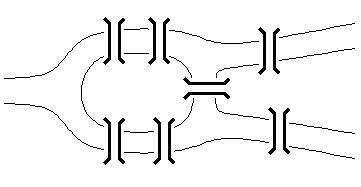
\includegraphics[width=0.4\textwidth]{konigsberg.jpg}
$\qquad \to\qquad$
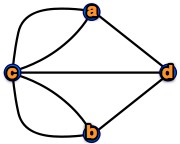
\includegraphics[width=0.3\textwidth]{konigsberg_graph.jpg}

Each land parcel is represented by a vertex (labelled with a letter) and each edge represents one of Koninsberg's seven bridges.

Does there exist a walk which uses every edge exactly once?

\subsubsection{Eulerian circuit}
\textbf{Defintion}: A circuit in a graph using every edge exactly once.

In a circuit, every time we visit a vertex, we use two edges incident to this vertex.

A graph is called \textbf{connected} if there is a path (or walk) between any pair of vertices.

\textbf{Theorem}: A connected graph contains an Eulerian circuit if and only if every vertex in it has an even degree. % lol like a bauss

\textbf{Proof}: We already established the "only if" part of the statement, now for the if part.

\textbf{"If" part}: Choose a circuit in our graph using as many edges as possible.
\begin{comment}
\begin{figure}[h]
\centering
\begin{tikzpicture}[scale=0.75,transform shape]
  \Vertex[x=0,y=2](1)
  \Vertex[x=1,y=3](2)
  \Vertex[x=3,y=0](3)
  \Vertex[x=4,y=2](4)
  \Vertex[x=3,y=3](5)
   \Vertex[x=5,y=2](6)
  \tikzstyle{LabelStyle}=[fill=white,sloped]
  \Edge(1)(2)
  \Edge(2)(3)
  \Edge(3)(4)
  \Edge(4)(5)
  \Edge(5)(1)
  \tikzstyle{EdgeStyle}=[bend left]
  \Edge(1)(2)
  \Edge(1)(3)
  \Edge(2)(5)
  \tikzstyle{EdgeStyle}=[bend right]
  \Edge(3)(4)
  \Edge(4)(5)
\end{tikzpicture}
\end{figure}
\end{comment}
If it uses all of the edges, this is an Eulerian circuit. 

If not, there exists an edge not in our circuit, and because the graph is connected, we can choose an edge incident to some vertex of this circuit.

Every vertex is incident to an even number of edges not in the chosen circuit.

Starting with the original edge, we can construct a walk using only edges not belong to the circuit.

We can continue until we reach the vertex we started at, i.e., we constructed a circuit, say $C'$, which contains no edges of $C$, but shares a vertex $v$ with the original circuit C.

We can trace $C$ (starting and ending at $v$), and then trace $C'$, so $C \cap C'$ also correspondings to a circuit, contradicting the choice of $C$.

\subsubsection{Eulerian Walk}
An \textbf{Eulerian walk} is a walk (not necessarily closed) which uses every edge exactly once.

\textbf{Corollary}: A connected graph has an Eulerian walk if and only if it has at most two vertices of odd degree.

\textbf{Proof}:
\begin{itemize}
\item \textbf{"Only if"}: Let an Eulerian walk start at $u$ and end at $v$. If $u = v$, this is an Eulerian circuit, so by the theorem, all degrees are even. If $u \neq v$, add an edge to the walk, and the graph. We have an Eulerian circuit in the new graph, so all degrees are even, so only $u \& v$ had an odd degree before.
\item \textbf{"If"}: If all degrees are even, we are done. If exactly two vertices $u \& v$ have an odd degree, add an edge $u\--v$. In the new graph, there is an Eulerian circuit, which corresponds to an Eulerian walk in the original graph.
\end{itemize}

A \textbf{Hamiltonian cycle} is a cycle in a graph that uses all of the vertices. The problem of determining whether a graph has a Hamiltonian circuit is \textbf{NP-complete}. (if $P \neq NP$, it is not possible to find Hamiltonian circuits efficiently)

\subsubsection{The Petersen graph}

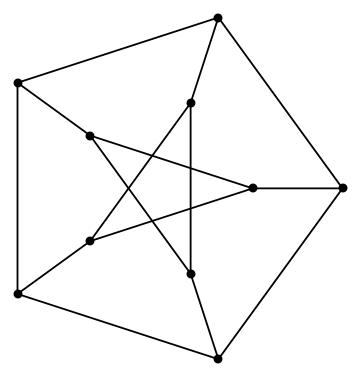
\includegraphics[width=0.3\textwidth]{petersen.jpg}

This graph has no Hamiltonian cycle. 

A graph is \textbf{3-regular} of every vertex has degree 3. 

A \textbf{3-edge colouring} of a 3-regular graph is a way of assigning colours $\{1, 2, 3\}$ to the edges of the graph so that every vertex is incident to the edges of all 3 colours. If a 3-regular graph has a Hamiltonian cycle, then it has a 3-edge colouring (use colours 1 and 2 on the cycle)

However, the Petersen graph does not have a 3-edge colouring. Suppose there is a 3-edge colouring.

\begin{enumerate}
 \item There is an edge of every colour on the outer cycle.
 \item It follows that the inner cycle has at least two edges of every colour, but there are 3 colours and only 5 edges.
\end{enumerate}

% November 18th

\subsubsection{Hamiltonian Cycles}

A cycle which uses every vertex exactly once. 

\textbf{Complete graph on n vertices $K_n$} 

Example:$K_s$ a graph where every pair of vertices is joined by an edge 

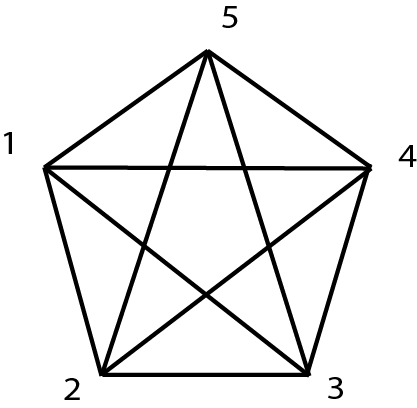
\includegraphics{fig13.png}

$K_n$ has $n$ vertices ${n \choose 2}$ edges = $\frac{n(n-1)}{2}$.

\textbf{Complete Bipartite graph $K_{n_1, n_2}$}

A complete bipartite graph $K_{n_1, n_2} = (V,E)$

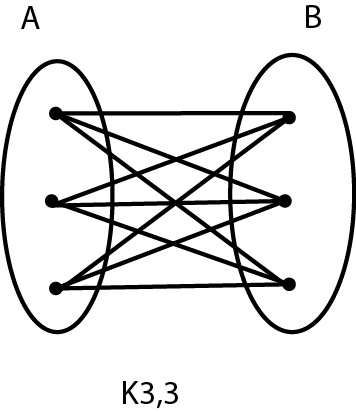
\includegraphics{fig14.png}

$V = A \cup B \qquad A \cap B = \emptyset \qquad |A| = n_1 \qquad |B| = n_2$ 

Every vertex of A is joined to every vertex of B and there are no other edges ($n_1 n_2$ edges in total)

If $n_1, n_2 \geq 2$, $K_{n_1,n_2}$ has a Hamiltonian cycle if and only if $n_1 = n_2$ (the vertices of the parts A $\&$ B must alternate along the cycle). 


\textbf{Theorem (Dirac):} Let G be a simple graph on n vertices, $n \geq 3$, then if $deg(v) \geq \frac{n}{2}$ for every vertex v of G then G has a hamiltonian cycle.

\textbf{Proof:} Assume that G does not have a Hamiltonian cycle. Further, assume that G has as many edges as possible subject to all of the above (Adding an edge between any pair of non-adjacent vertices of G creates a Hamiltonian cycle.)

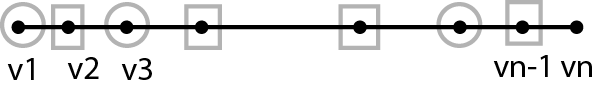
\includegraphics{fig15.png}

There are $\geq \frac{n}{2}$ squares neighbours of $v_i$

Let the circles in the picture denote vertices to the left of the squares.

There are $\geq \frac{n}{2}$ circles. If $v_n$ is adjacent to one of these vertices say $v_k$ then: $v_1 \to v_k \to v_n \to v_{k+1} \to v_1$ is a hamiltonian cycle. So we may assume that $v_n$ is adjacent to any of these vertices.

So there are only $n - 1 - \frac{n}{2} < \frac{n}{2}$ vertices which $v_n$ can be adjacent to $\to$ contradiction $\blacksquare$

Example:
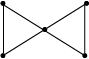
\includegraphics{fig16.png}

$deg = \lfloor n / 2 \rfloor \to$ No hamiltonian cycle. 

\section{Trees (section under construction)}
A \textbf{tree} is a connected simple graph without any cycles.

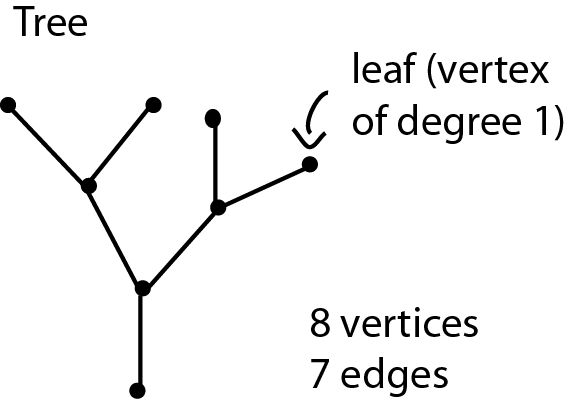
\includegraphics{fig17.png}

\textbf{Theorem:}
\begin{enumerate}
    \item In a tree there exists a unique path between any pair of vertices.
    \item Deleting any edge from a tree disconnects it.
    \item Adding an edge between non-adjacent vertices of a tree to a tree creates a cycle.
    \item If a tree has at least $\geq 2$ vertices then it has $\geq 2$ leaves.
    \item The number of edges in a tree is one less then the number of vertices.
\end{enumerate}

\textbf{Proofs for the above:}
\begin{enumerate}
    \item Suppose not, for some pair of verties $x$, $y$ there exist two paths between them. Let $p_1$, $p_2$, denote those paths. Let $x^{'}$ be the first vertex where $p_2$ deviates from $p_1$. Let $y^{'}$ be the next vertex along $p_1$ which belongs to $p_2$. 
    Then, if $x^{'} \to(p_2)\to y^{'} \to(p_1) \to x^{'}$ is a cycle $\to$ contradiction
    \item If we delete an edge $e = \{x, y\}$. e was the edge of the unique path from $x$ to $y$ after deleting it there are no paths from x to y $\checkmark$ 
    \item Adding an $x\-- y$ edge together with the existing path from x to y in a tree creates a cycle.
    \item Considering the longest path in a tree, then x and y are both leaves.
    \item Induction on the number of vertices.\\
    \textbf{Base case}:1 vertex three has no edges\\
    \textbf{Induction step:} Consider a tree on $(n+1)$ vertices. Let $v$ be a leaf of this tree. Delete $v$ (this removes 1 vertex and 1 edge). The remaining graph clearly has no cycles and is connected. (no path without an end in v can use v).\\
    By the induction hypothesis it has $n$ vertices and $n-1$ edges so our graph had $n$ edges. $\blacksquare$
\end{enumerate}

% November 21st
\subsection{Counting trees}
How many different trees are there with n vertices?

V = \{0,1,2\}

\textbf{Unlabeled Trees}

$G_1 = (V_1, E_1), \quad G_2 = (V_2, E_2)$ - simple graphs

$G_1$ and $G_2$ are \textbf{isomorphic} if there exists $f:V_1 \to V_2$ a bijection, such that $u \-- v \in E_1$ if and only if $f(u)\-- f(v) \in E_2$. In other words, two nodes in the first tree that are connected by an edge correspond to nodes in the second tree that are connected by an edge and vice-versa.

How many different (non-isomorphic) trees are there?

n =1 , n = 2

There is no closed form expression of the \# of unlabeled trees.

\textbf{Labeled trees}

How many trees are there with the vertex set V =\{0,1,2,\ldots, n-1\}? (what about simple graphs?)

There are $\displaystyle {n \choose 2}$ possible edges and $\displaystyle 2^{{n \choose 2}}$ different simple graphs.

\begin{itemize}
\item n = 1: 1 way
\item n = 2: 1 way
\item n = 3: 3 ways
\item n = 4: 4 ways to label linear tree, 24 ways to label the non-linear tree if we fix the left end but this way we count every tree twice so $24/2$. $12 + 4 = 16$
\end{itemize}

\subsubsection{Number of labeled trees}

\textbf{Theorem (Cayley)}: There are $n^{n-2}$ labeled trees with n vertices. 

How can we represent trees in the computer?

\textbf{Adjacency matrix}

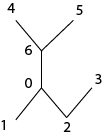
\includegraphics{fig1.png} 
$\qquad$can be represented by the adjacency matrix:

$$
\begin{matrix}
0 & 1 & 1 & 0 & 0 & 0 & 1 \\
1 &0 & 0 & 0 & 0 & 0 & 0 \\
1 & 0 & 0 & 1 & 0 & 0 & 0 \\
0 & 0 & 1 & 0 & 0 & 0 & 0 \\
0 & 0 & 0 & 0 & 0 & 0 & 1 \\
0 & 0 & 0 & 0 & 0 & 0 & 1 \\
1 & 0 & 0 & 0 & 1 & 1 & 0 \\
\end{matrix}
\qquad \begin{cases}
1 $ if and only if corresponding vertices are adjacent$ \\
0 $ otherwise$\\
\end{cases}$$

$\to {n \choose 2}$ bits

There is no way to represent a general graph with fewer bits. But for trees we can do better. 

\textbf{The Incidence List}: A tree has $n-1$ edges. Let us write down the ends of the edges.

$
\begin{pmatrix}
0 & 0 & 0 & 2 & 4 & 5 \\
1 & 2 & 6 & 3 & 6 & 6 \\
\end{pmatrix}
\to$
a sequence of $2(n-1)$ numbers (takes $2(n-1)\lceil log_2 n \rceil$ bits)

There are at most $n^{2(n-1)}$ labeled trees on n vertices.

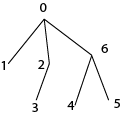
\includegraphics{fig2.png}

\textbf{The Parent List}:  For every vertex (except the root) there exists a unique edge from it along the path towards the root. 
We call the second end of this edge the \textbf{parent} of the vertex. 
Every edge joins some vertex to its parent.

$\begin{matrix}1 & 2 & 3 & 4 & 5 & 6 \\0 & 0 & 2 & 6 & 6 & 0\end{matrix}$.

The second row completely records the tree as the first row is just $0$ to $n$ in order $\leq n^{n-1}$ trees

Every tree corresponds to a parent list, but the converse is not true. Example:

$\begin{matrix} 1 & 2 & 3 & 4 & 5 \\2 & 3 & 1 & 5 & 4 \end{matrix}\qquad$ corresponds to a disconnected non-simple graph.

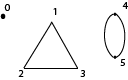
\includegraphics{fig3.png}

\textbf{Pr\"{u}fer codes}

At each step we record the leaf with the smallest label, we record its parent and then we erase the leaf and recurse (extended Pr\"{u}fer code).

$\begin{matrix}
1 & 3 & 5 & 2 & 6 & 8 & 7 & 4 & 9 \\
2 & 2 & 2 & 0 & 7 & 7 & 4 & 0 & 0 \\
\end{matrix}$

$2(n-1)$ numbers

It is possible to reconstruct the first row from the second one. 

\textbf{Justification:}
$i^{th}$ entry of the $1^{st}$ row is the smallest number which is not yet in the $1^{st}$ row, and does not appear in the $2^{nd}$ row in the $i^{th}$ or greater position.

Furthermore, we do not need the last column since the last vertex will always be 0 (the root).

Every tree can be recorded as a sequence of $n-2$ numbers.

%November 23rd

\includegraphics{prufer.png}

\textbf{Cayley's theorem}: There are $n^{n-2}$ labeled trees on $n$ vertices.

\textbf{Proof}: Prufer codes

1 3 5 2 6 8 7 4 9 $\to$ Extended Prufer code

2 2 2 0 7 7 4 0 0 $\to$ Prufer code

% I noted them down on my notebook, will convert later
% I think you missed the first tree though, by the time he came in, it was erased already. (the one on the right blackboard?
% No, there was another tree on the left with the above Prufer code ^ I only got part of it though, but I'll calculate it out later. Gotcha

\paragraph{Reconstructing extended Prufer code from the Prufer code}

\begin{enumerate}
\item Last digit of the 2nd row is 0
\item Every entry of the first row is the smallest (non-zero) number that does not appear to the left of it in the 1st row or underneath and to the right in the 2nd row (there is always a choice)
\end{enumerate}
\textbf{Example}: Tree with 9 vertices. Prufer code: 7 numbers from 0 to 8

$\begin{matrix}
2 &3& 4& 1& 6& 7& 8 &5\\
4 &5& 1& 7& 7& 0& 5& 0
\end{matrix}
$

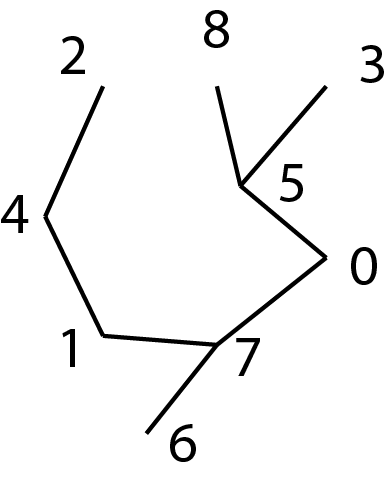
\includegraphics{fig5.png} 

Every Preufer code corresponds to a graph with $n-1$ edges and $n$ vertices

[picture of connections between first row] $\to$ Every vertex (except for 0) is joined to exactly one vertex to the right of it.

\subsubsection{Number of unlabeled trees}

\textbf{Unlabeled trees}: let $T_n$ be the number of unlabeled trees on $n$ vertices $T_1 = T_2 = T_3 = 1, \quad T_4 = 2, \quad T_5 = 3$ (draw them out to see)

\textbf{Theorem:}

$$\displaystyle \frac{n}{n!} \leq T_n \leq 2^{2(n-1)} = 4^{n-1}$$

\subsubsection*{$\to$ Lower bound on the number of unlabeled trees}

$$\displaystyle \underbrace{n^{n-2}}_{\text{\# of labeled trees}} \leq \underbrace{n! \cdot T_n}_{\substack{\text{\#of ways of labeling} \\ \text{unlabeled tree}}}$$

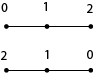
\includegraphics{fig6.png}

Each unlabeled tree can be labeled in at most $n!$ ways. Since the number of labeled trees is $n^{n-2}$, the number of unlabeled trees is at least $\frac{n^{n-2}}{n!}$

\subsubsection*{Stirling's formula}

$\displaystyle n! \approx \sqrt{2\pi n} (\frac{n}{e})^n$

$\displaystyle \lim_{n \to \infty} \frac{n!}{\sqrt{2\pi n}(\frac{n}{e})^n} = 1$

$\displaystyle \frac{n^{n-2}}{n!} \approx \frac{n^{n-2}}{\sqrt{2 \pi n}\frac{n^n}{e^n}} = \frac{e^n}{\sqrt{2 \pi}n^{5/2}} = \frac{1}{\sqrt{2 \pi}}n^{-5/2}e^n$

\subsubsection*{$\to$ Upper bound on the number of unlabeled trees}
$$T_n \leq 2^{2(n-1)} = 4^{n-1}$$

Trace the tree drawn in the plane. It takes 2(n-1) steps, at each step, let us record 1 if we go away from the root and 0 if we go towards the root. 

The tree is completed described by a sequence:

1 1 1 0 1 0 0 1 0 0

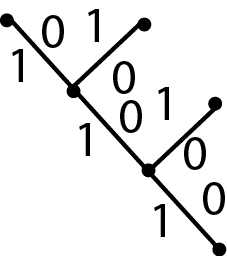
\includegraphics{fig7bis.png}

Another example:

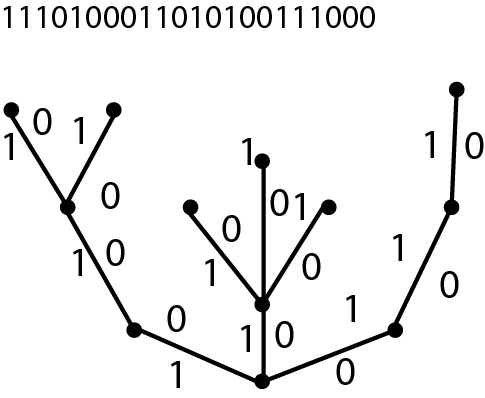
\includegraphics{fig7.png}

There are $n-1$ edges in a tree and each edge must be recorded by a 0 and a 1. The length of the sequence is therefore $2(n-1)$. There are $2^{2(n-1)} = 4^{n-1}$ such sequences.

Note that a sequence of 0's and 1's does not necessarily produce a tree. Example: 1 1 0 0 0 1 1 0

$\underbrace{11000}_{\text{in every initial segment the \# 1's must be at least as large as the \# of 0's}}110$

Furthermore, there must be an equal number of 0s and 1s.

\subsection{Minimum cost (or spanning) tree}

We have n cities, 8 want to build a road netwrok connecting them. We want to be able to get from every city to every other city possibly passing some cities in between. We know costs (on distances) for building roads between cities. How can we build the network spending as little as possible.

Let $d \ : \ \{0,1,\ldots,n-1\} \times \{0,1,2,\ldots,n-1\} \to \mathbb{R}_+$ be the distance function $d(0,1) = 1 \qquad d(1,2) = 2 \ldots$

We want to construct a tree on these n vertices, with the sum of distances over its edges as small as possible.

Enumerating all the trees takes too much time.

\textbf{Greedy algorithm:} "Be as greedy as possible at each step." At each step of the algorithm build the road which is as cheap as possible (i.e. connects two cities at the shortest distance) joining two cities not connected by the network.

%November 25th

Given a weighted graph $G = (V, E)$ find a spanning tree:

$T = (V, S) \ \mathrm{of} \ G \ \mathrm{with} \ \sum_{e \in S} d(e) \ \text{minimum}$

\textbf{Kruskal's (Greedy) algorithm}

\includegraphics{kruskal.png}

Grow $S$ step by step. Start with $S = \emptyset$. At each step add to $S$ an edge of $G$ with the minimum weight (value of $d$) so that the graph formed by edges in $S$ remains acyclic.

(If $G$ was connected this algorithm produces a tree, if not we can add edges)

\textbf{Theorem}: Kruskal's algorithm produces a minimal cost tree.

\textbf{Proof}: We will prove by induction on the $\#$ of steps performed that $S$ belongs to some minimum cost tree. (This suffices)

\textbf{Base case}: In the beginning, $S = \emptyset$.

\textbf{Induction step}: By the induction hypothesis $S$ belongs to some MCT $T'$, we add an edge $e$ to $S$. Our goal is to show that $S \cup \{e\}$ belongs to some MCT.

\begin{itemize}
\item \textbf{Case 1}: $e$ belongs to T (the edge of set of $T'$), then so does $S \cup \{e\}$, and we are done.
\item \textbf{Case 2}: $e$ does not belong to $T'$. Adding $e$ to $T'$ creates a cycle C. Is it possible that all edges of C belong to S? No, because in our algorithm S never contains any cycles. 
So consider $e'$ in C, $e' \notin S$. We added $e$ and not $e'$  so $d(e') \geq d(e)$.\\
Consider deleting $e'$ from $T'$ and adding $e$.
\end{itemize}
\textbf{Proof:} We end up with a new tree. The cost of this tree is  minimal.
% where is the above sentence? it was on the blackboard 

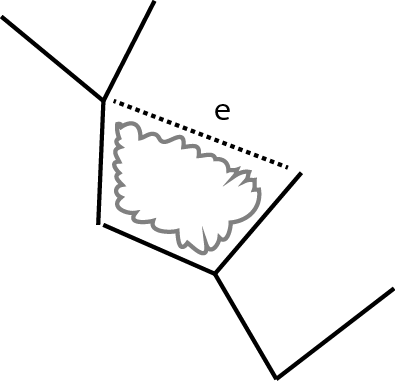
\includegraphics{fig9.png}

\section{Planar graphs}

Graphs which can be drawn in the plane without crossings.

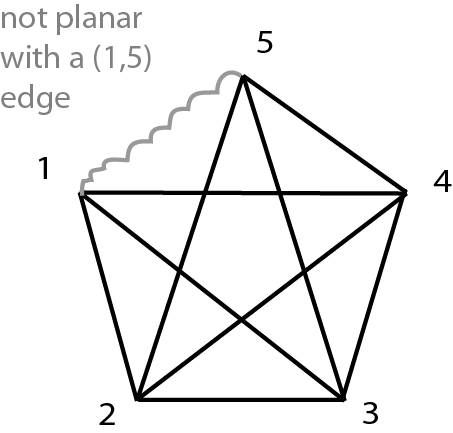
\includegraphics{fig10.png}
$\to$
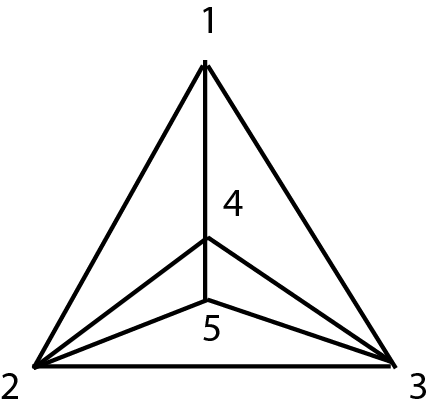
\includegraphics{fig11.png}

\textbf{Theorem (Fary 48):} A planar graph always has a drawing where all the edges are represented by straight lines.

If a graph is drawn on the plane, it partitions it into regions called \textbf{faces}.

\textbf{Theorem (Euler's formula)}: Let G be a connected graph drawn in the plane with $n$ vertices, $m$ edges and $f$ faces then $f = m -n + 2$

\textbf{Proof}: By induction on the number of edges $m$ 

\textbf{Base case}: 0 edges $\to 1$ vertex $\to 1$ face $\checkmark$

\textbf{Induction step}: We are assuming that the formula holds for all graphs with $< m$ edges.
\begin{itemize}
\item \textbf{Case 1}: $G$ has no cycles $\to G$ is a tree. There is one face and $m = n -1 \to 1 = (n-1) - n+2  \quad \checkmark$

\item \textbf{Case 2}: G has a cycle C. Delete an edge of C. The two sides of the deleted edge belonged to different faces. Deleting $e$ decreases the number of faces by 1. \\
By the induction hypothesis:
$(f - 1) = (m - 1) - n + 2 \quad \checkmark$
\end{itemize}


%% November 28th
\textbf{Example:}

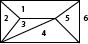
\includegraphics{fig18.png}

6 vertices = n\\
10 edges= m\\
6 faces = f

What is the maximum number of edges in a  planar simple graph with n vertices?

\textbf{Euler's formula} n -m + f = 2 for every planar graph

\textbf{Theorem:} A planar graph on $n$ vertices has edges $m \leq 3n-6$ (can be achieved for all $n \geq 3$)

\textbf{Proof:}
\begin{itemize}
    \item Every edge belongs to at most two faces (1)
    \item Every face is bounded by at least 3 edges (2)
\end{itemize}
Count pairs (edge, face) such that the edge belongs to the face.

Say there are L such pairs.

$
\begin{cases}
L \leq 2m$ from (1) $\\ 
L \geq 3f$ from (2) $\\
\end{cases}
\to 3f \leq 2m$ 
% is that \subseteq or geq? yeah we're talking about numbers not sets lol ok

$3(m-n+2) \leq 2m$

$m -3n + 6 \leq 0$

$m \leq 3n - 6$

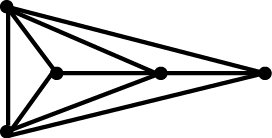
\includegraphics{fig19.png}

This is a complete graph on 5 vertices with one edge deleted. 

\textbf{Corollary}: $K_5$ is not planar

10 edges 5 vertices $\qquad 10 > 3 \cdot 5 - 6$

\includegraphics{fig20.png}

A \textbf{subdivision} of a graph G is a graph obtained from G replacing some of the edges by paths, that is dividing those edges using new vertices of degree 2.

Clearly a subdivision of a non-planar graph is non-planar. So any graph with a subdivision of $k_5$ as a subgraph is non planar.

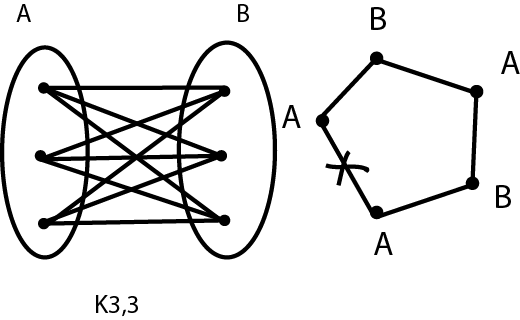
\includegraphics{fig21.png}

\textbf{Bipartite graphs:} A graph $G = (V,E)$ is bipartite if there exists a partition $V = A \cup B$, $A \cap B = \emptyset$ so that every edge joins a vertex of A to a vertex of B.

(In a bipartite graph every cycle has even length). In particular, it has length $\geq$ 4.

\textbf{Theorem}: $m \leq 2n - 4$ for a planar simple bipartite graph $G$ with $n$ vertices and $m$ edges. $n \geq 4$

\textbf{Proof:} 
\begin{itemize}
\item Every face contains at least 4 edges\\
\begin{flalign*}
2m &\geq 4f \to m \geq 2f &\\
m &= n+f-2 \leq n +\frac{m}{2} - 2 &\\
2m &\leq 2n + m - 4 &\\
m &\leq 2n-4&\\
\end{flalign*}
\item **missed**
\end{itemize}

\textbf{Theorem (Kuratowski):} A graph G is non-planar if and only if it contains a subdivision of $K_5$ or $K_{3,3}$ as a subgraph.

Being planar is in NP $\to$ a drawing is a certificate.

Being non-planar is also in NP $\to$ a subdivision of $K_5$ or $K_{3,3}$ is a certificate.

It is possible to test planarity very efficiently (in fact, in linear time $O(n)$)

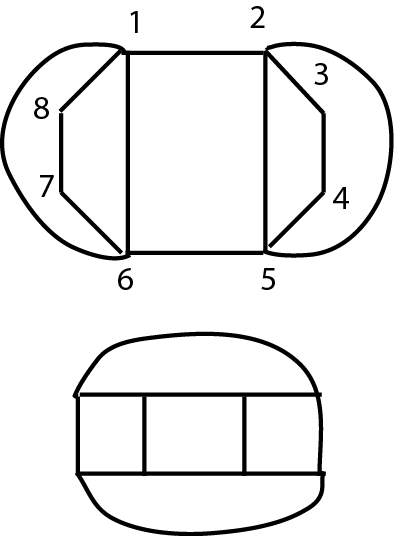
\includegraphics{fig22.png}
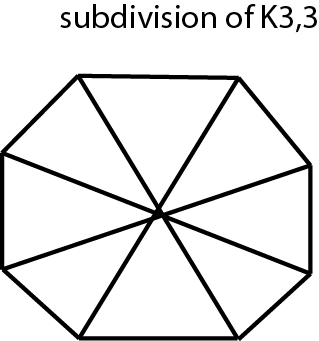
\includegraphics{fig23.png}

\subsection{Coloring graphs}

A \textbf{(proper) k-coloring} of a graph $G = (V, E)$ is a function $c : V \to \{1, 2, \ldots, k\}$ so that $c(u) \neq c(v)$ for every pair of adjacent vertices $u,v \in V$.

\textbf{Chromatic number}: $\chi(G)$ of a graph $G$ is the smallest positive integer $k$ such that $G$ allows a k-coloring.

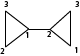
\includegraphics{fig24.png}

x(G) = 3
x(G) $\geq$ 3 $\to$ 2 is not enough.
x(G) $\leq$ 3 (just color the graph to show)

\paragraph{Graph coloring}

\textbf{k-coloring}: c - V $\to$ $\{1, 2, \ldots k\}: c(u) \neq c(v)$ if $u$ is adjacent to $v$

$X(G)$ [chromatic number] \-- minimum $k$ such that $G$ can be k-colored.

[$X(G) = 1$ if and only if $G$ has no edges]
When is $X(G)$ = 2?

G is \textbf{bipartite} if $V$ can be partitioned:

$V = A \cup B$
$A \cap B = \emptyset$

so that every edge joins a vertex of $A$ to a vertex of $B$.

\textbf{Claim}:

A graph is 2-colorable if and only if it is bipartite.

A graph is not bipartite if it contains an odd cycle (a cycle with an odd number of vertices).

\textbf{Theorem}: A graph is bipartite (or two-colorable) if and only if it contains no odd cycles.

\textbf{Proof}: A graph is not bipartite if and only if it contains an odd cycle.

We already know the 'if' part, so it only remains to show the 'only if' part.

Suppose that $G$ is not bipartite (or two-colorable), we may assume that $G$ is connected. Let V be some vertex of $G$. 

Let $d(u,v)$ denote the length of the shortest path between $u$ and $v$ for any other vertex $u$. Color $v$ in color 1, and color every other vertex $u$ in color 1 if $d(u,v)$ is even, and color 2 if $d(u,v)$ is odd

This doesn't produce a two coloring. So there are adjacent vertices $u_1$ and $u_2$ of the same color.

$d(x, v)$ - differ by at most 1
$d(y, v)$ 

\includegraphics{something.png}

This is the closest vertex to $u_1$ and $u_2$ along the shortest paths along the shortest paths from $u_1$ and $u_2$ to $v$ to belongs to both paths.

$d(u_1,v) = k_1 + L$
$d(u_2,v) = k_2 + L$
$k_1 = k_2 = k$

[BOTTOM OF FIGURE] - an odd cycle of length 2k.

The problem of determining whether $X(G) \leq 3$ is NP-hard (at least as hard as every problem in NP)

\subsection{What obstructions are there to k-coloring?}

$K_{k+1}$ as a subgraph $\to$ There exist non k-colorable for any k with [missing]?

\textbf{Theorem (Brooks)}: If a graph has maximum degree $k$ then it is $(k+1)-colorable$.

\textbf{Proof}: By induction on the number of vertices.

\begin{itemize}
    \item \textbf{Base Case:} (1 vertex) $\checkmark$
    \item \textbf{Induction Step:} Let G be a graph with n+1 vertices. Choose some vertex v in G and remove it. The graph that remains has n vertices, has maximum degree $\leq k$ so is $(k+1)$-colorable by the induction hypothesis.

\end{itemize}

Neighbors of $v$ use at most $k$ colors, so there is at least one color that is not yet used, and we can color $v$ in this color.

\subsection{Coloring of planar maps}: In a map every country is a contiguous region of the plane. We want to colour the map so that any two countries which share a border (non-zero length segment) receive different colors. How many colours suffice?

\textbf{The Four colour theorem:} Every map is 4-colourable (Francis Guthrie 1852). Appel \& Hakken published a non human-readable proof in 1976 (solved by computer-assistance using case-analysis)
 
\textbf{Dual graph}:
\begin{itemize}
    \item Vertices correspond to regions
    \item Two vertices are joined by an edge if regions share the segment of the border
    \item We get a planar graph.
    \item It now suffeces to show that $\chi(G) \leq 4 (\leq 5) for every planar (simple) graph G$
\end{itemize}


%% December 2nd

\section{Coloring planar graphs}

Four-colour theorem: $\chi(G) \leq 4$ for every planar (simple) graph G.

\textbf{Six-color theorem:} $\chi(G) \leq 6$

\begin{itemize}
\item \textbf{Claim:} Every planar simple graph contains a vertex of degree $\leq 5$
\item \textbf{Proof of thTe claim:} $\sum_{v \in V} deg(v) = 2e \leq 2(3n-6) = 6n -12$\\
Suppose the graph has $n$ vertices\\
$$\displaystyle \frac{\sum_{v \in V} deg(v)}{n} \leq 6 - \frac{12}{n} < 6$$
\item \textbf{Proof of the 6-color theorem:}
By induction on the number of vertices in G. 
\begin{itemize}
\item \textbf{Base case:} 1 vertex $\checkmark$
\item \textbf{Induction Step:} Let $v$ be a vertex of degree $\leq 5$ in G. By the induction hypothesis if we delete $v$ from $G$ we can colour the vertices in 6 colours, but then we can also colour v, because at most 5 colours are used on its neighbours.
\end{itemize}

\textbf{Proof of the 5-color theorem:} $\chi(G) \leq 5$
\includegraphics{fig40.png}

Note: $K_6$ is not 5-colorable but every vertex has degree 5.

\textbf{Proof:} By induction as the previous theorem.

\begin{itemize}
\item \textbf{Base case}: same as before
\item \textbf{Induction step}: Let $v$ be the vertex of the smallest degree in $G$.
    \begin{itemize}
    \item \textbf{Case 1}: $deg(v) \leq 4 \to$ then the argument from the 6 colour theorem works.
    \item \textbf{Case 2}: $deg(v) = $%%%%
    \item The new graph can be coloured in 5 colours by the induction hypothesis. Let $u_1 \& u_3$ inherit the colour of the new vertex in the smaller graph. Neighbours of v now receive at most 4 colours, so there is a colour available for $v$.\\
    The only possible difficulty in this step is that $u_1 \& u_3$ are adjacent. But we could have chosen any pair of neighbours of $v$ instead. There exists some pair of non-adjacent neigbours as otherwise $G$ would have contained a subgraph isomorphic to $K_5$.
    \end{itemize}
\end{itemize}
\end{itemize}

\textbf{3-edge coloring of a graph with all vertices of degree 3} $\to$ cubic graphs 

Coloring of edges in colours 1,2,3 so that every vertex is incident to an edge in every colour.

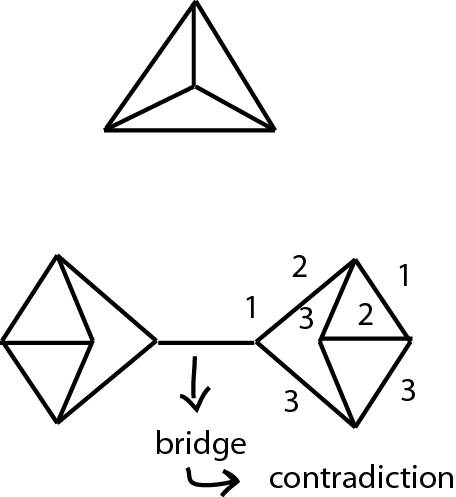
\includegraphics{fig42.png}

A \textbf{bridge} in a graph is an edge so that deleting it disconnects the graph.

\textbf{Theorem:} Every cubic planar graph with not bridges can be 3-edged colored.

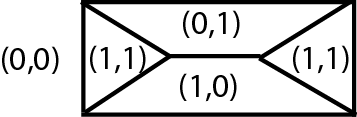
\includegraphics{fig43.png}
\textbf{Proof:} By the 4.C.T. the faces of the graph can be coloured in 4 colours. (0,0), (0,1), (1,0), (1,1)
Now we assign colours to edges (0,1),(1,0),(1,1). If an edge forms a border of regions with colours $(a_1, b_1) \& (a_2, b_2)$ we give it colour $(c,d)$ so that:
\begin{itemize}
    \item $c = 0$ if $a_1 = a_2$ and $c= 1$ otherwise
    \item $d = 0$ if $b_1 = b_2$ and $d = 1$ otherwise
    \item No edge receives a (0,0) colour.\\
    Why no two edges incident to the same vertex receive the same colour?\\
    TWo edges of the same colour would imply that two faces have the same colour.
\end{itemize}


%%% December 5th

%lecture 39 2011-12-05
\section{Review}

\subsection{Bijective proofs of combinatorial formulas}

Find a bijective proof of ${n \choose r}{r \choose k} = {n \choose k}{n - k \ choose r -l}$

For $n \leq r \leq k$.

$[n] = \{1, 2, \ldots , n\}$

$A \in [n], |A| = r, B \in A, |B| = k$

We can think of the left side as counting the pairs of subsets (A, B):

$\{(A, B): |A| = r, |B| = k, B \in A \in [n]\}$

That is the set that is counted on the left.

\includegraphics{figure1.png}

We can think of the right side as counting the pairs of subsets (C, D):

$\{(C, D): |C| = k, |D| = r - k, C \cap D - \emptyset, C, D \leq [n]\}$

This is the set that is counted on the right.

\includegraphics{figure2.png}

We want a bijection $f$ such that:

$f: (A, B) \to (B, A - B)$ 

maps the pairs from "the left side" to pairs on "the right side".

$(C, D) \to (C \cup D, C)$ 

is an inverse map, so $f$ is a bijection.

\subsection{Example problem from final}

Prove ${2n \choose n} + {2n \choose n + 1} = \frac{1}{2}{2n + 2 \choose n + 1}$

$\frac{\cancel{(2n)!)}}{n!n!} + \frac{\cancel{(2n)!}}{(n+1)!(n+1)!} = \frac{1}{2} \frac{(2n+2)!}{(n+1)!(n+1)!}$

$\cancel{(n+1)}(n+1) + \cancel{(n+1)}(n) = \cancel{\frac{1}{2}}(2n + 1)\cancel{(2n + 2)}$

$(n + 1) + n = 2n + 1 \checkmark$
% will rewrite algebra out later

Find a bijective proof of the above combinatorial equation:

\includegraphics{figure3.png}

${2n + 2 \choose n + 1} = \underbrace{{2n \choose n - 1}}_{\text{Number of ways of selecting of the last two elements}} + \underbrace{2 {2n \choose n}}_{\text{Number of ways of selecting one of the last two elements}} $

Dividing by half:

$\frac{1}{2} {2n + 2 \choose n + 1} = {2n \choose n} + \frac{1}{2}({2n \choose n - 1} + {2n \choose n + 1} = {2n \choose n} + {2n \choose n+1}$

\subsection{Another problem}

$\displaystyle \sum_{i=0}^{k} {n + i \choose n} = {n + k + 1 \choose n + 1}$

This is selecting a $(n+1)$ element subset out of the set of size $(n + k + 1)$.

\includegraphics{figure4.png}

Consider the position of the last selected element. It is between the $(n+1)^{st}$ and $(n + k + 1)^{st}$ position, so it is position is $n + i + 1$ for $0 \leq i \leq k$

There are ${n + i \choose n}$ ways of selecting the other $k$ elements.

\subsection{Logic}

Know how to prove logical formulas using the rules of logic or logic tables.

\textbf{Example}:

Show $(p \wedge (p \to q)) \to q$ is a tautology.

% I don't know how to latex tables :(
\begin{tabular}{ |c |c| c| c| c| }
p & q & $p \to q$ & $p \wedge (p \to q)$ & $(p \wedge (p \to q)) \to q$ \\
\hline
1 & 1 &   1   &         1        &         1 \\
1 & 0 &   0   &         0        &  1 \\
0 & 1 &   1   &         0        &  1 \\
0 & 0 &   1   &         0        &  1 \\
\end{tabular}

Show that $P \lor (q \to r)$) is equivalent to $q \to (p \lor r)$

Now $p \lor ((\lnot q) \lor r) \Leftrightarrow \lnot q \lor (p \lor r)$ by communitativy and associativity of v

Write down the negation of $\forall n \in \mathbb{N}((n^3 + 6n + 5$ is odd $)\to ($n is even$))$

So bascially $\forall n \in \mathbb{N}(p(n)) \exists n \in \mathbb{N} \lnot ((n^3 + 6n +5)$ is odd$) \to($ n is even$))$

Negation is $\exists n \in \mathbb{N} (\lnot p(n)) \exists n \in \mathbb{N}((n^3 +6n + 5)$ is odd $) \wedge (n$ is odd$)) \to$ false

$n \equiv 1 (mod \ 2) \to$ odd
$n^3 \equiv 1 (mod \ 2)$
$n^3 + 6n + 5 \equiv 1 + 0 + 1 \equiv 0 (mod \ 2)$

\subsection{Number theory review}

Euclid's algorithm not on the final because it was on the midterm?

\textbf{Fermat's Little Theorem}: $a^{p-1} \equiv 1 (mod \ p)$ for all primes $p, p \nmid a$

Compute $302^{303} (mod 11)$

$302 \div 11 = 27$ remainder $5$

$302 \equiv 5 (mod \ 11)$
$302^{302} \equiv 5^{302} = 5^{300} \cdot 5^2 = (5^{10})^{30} \cdot 5^2 \equiv 5^2 = 25 \equiv 3 (mod \ 11)$

%%% December 6th

Show that for every prime $p$ and integer $k \qquad 1 < k \leq p$ 

(a)

$p | {p \choose k}$

${p \choose k} = \frac{p!}{k!(p-k)!} \to$ the numerator is divisble by $p$ and the denominator is not divisible by $p$ so the ratio is divisible by $p$ (only true for primes)

(b)

Show that the product of all primes strictly between $n$ and $2n$ is no greater than ${2n \choose n} = \frac{(2n)!}{n! \ n!}$

By the same argument as in ${2n \choose n}$ is divisible by every prime $p: \quad n < p \leq 2n$

So the product of these primes divides ${2n \choose n}$, so it's at most ${2n \choose n}$

Show that

$\displaystyle \sum_{k=0}^n k(n-k) = {n+1 \choose 3}$

Proof by induction on $n$:

\begin{itemize}
    \item \textbf{Base case} (n=1): $0 \cdot 1 + 1 \cdot 0 = {2 \choose 3} \qquad \checkmark$
    \item \textbf{Induction step:} \\
    \begin{flalign*}
        \sum_{k=0}^{n+1} k((n+1)-k) = \sum_{k=0}^{n+1} k(n-k)+k &=\sum_{k=0}^{n+1} k(n-k) + \sum_{k=0}^{n+1} k &\\
         {n+1 \choose 3} &= \sum_{k=0}^{n} k(n-k) + (n+1)n(n-1) - (n+1) \text{ (by induction hypothesis)} &\\
    \end{flalign*}
    \begin{flalign*}
         & = \frac{(n+1)n(n-1)}{3!} - (n+1) + \frac{(n+1)(n+2)}{2} =? {n+2 \choose 3} = \frac{(n+2)(n+1)n}{3!} &\\
    \end{flalign*}
    \text{Multiply by 6}
    $n(n-1) - 6 + 3(n+2) = (n+2)n$\\
    $n^2 - n - 6 + 3n + 6 = n^2 + 2n \qquad \checkmark$\\
\end{itemize}

%%%% Show that $\displaystyle \sum_{k=0}^n$ oh well

Show that $\displaystyle \sum_{k=0}^n = \frac{n!2^k}{k! (n-k)!} = 3^n$

$\displaystyle \sum_{k=0}^n {n \choose k}2^k 1^{n-k}=3^n \qquad \sum_{k=0}^n {n \choose k}x^k y^{n-k} = (x+y)^n \qquad x = 2 y = 1$ (binomial theorem with x = 2 y = 1)

How many pairs of subset $A,B \subseteq \{1,2,3,4,5\}$ are there so that $A \subseteq B$

Product rule: Every element can
\begin{itemize}
    \item belong to neither $A$ nor $B$
    \item belong to $A$ and $B$
    \item belogn to just $B$ ($3^5$ choices in total $\to$ 243)
\end{itemize}

How many solutions are there to $x_1 + x_2 + x_3 + x_n = 30$ with $3 \leq x_i \leq 1$ and $x_i$ is an integer

$x_1 + x_2 + \ldots x_k = n$

it has ${n+k - 1 \choose k -1}$ non-negative integer solutions 

$(x_1 -3) + (x_2 -3) + (x_3 - 3) + (x_4 - 3) = 30 - 3 \cdot 4 = 18$

$y_i = x_i - 3$

$y_1 + y_2 + y_3 + y_4 = 18$

$0 \leq y_i \leq 7$ without and upper bound we have ${18 + 4 -1 \choose 4 -1} = {21 \choose 3}$

Let $A_i = \{\text{solutions with }y_i \geq 8 \}$

In total we have ${21 \choose 3} - |A_1 \cup A_2 \cup A_3 \cup A_4|$ solutions which satisfy the bound.

$|A_i| = {13 \choose 3} \qquad |A_i \cap A_j|$

$y_1 \geq 8 \to (y_1 - 8) + y_2 + y_3 + y_4 = 10 \qquad {10+3 \choose 3} = {13 \choose 3}$

$y_1 \geq 8, \quad y_2 \geq 8 \to (y_1 - 8) + (y_2-8) + y_3 + y_4 = 18 - 2 \times 8 = 2$

${21 \choose 3} \sum^4_{i=1} |A_i| + \sum_{1 \leq i < j \leq 4} |A_1 \cap A_j| = {21 \choose 3} - 4{13 \choose 3} + 6 {5 \choose 3}$

\textbf{Notes:}
Remember brufer codes, kruskal's algorithm and how to count anagrams (e.g. mississipi)

Let $G$ be a planar connected graph with every vertex of degree 3 and 46 vertices. We add 30 edges to $G$ arbitrarily.

How many edges and faces will there be in the resulting graph?

Twice the number of edges in $G = \sum \deg (V) = 46 \cdot 3 = 138$ 

number of edges = $\frac{46 \cdot 3}{2} = 23 \cdot 3 = 69 \to$ after adding 30 edges we get 99.
 
By Euler's formula: $F = E - V +2 = 99 - 46 + 2 = 55$

Does there exist a simple planar graph so that its edges can be coloured in colours red, blue and green so that every edge of every colour form a spanning tree (a tree on the same set of vertices).

\textbf{No.}A tree on $n$ vertices has $(n-1)$ edges. Three trees have $3 (n-1) = 3n-3$ edges in total. But a planar graph has at most $3n-6$ edges (for $n \geq 3$).

A \textbf{bridge} in a connected graph is an edge whose deletion disconnects the graph.

Show that a connected graph is a tree if and only if every edge is a bridge.

$\to$ If $G$ is a tree, consider an edge $u\--v$, there exists an unique pass between $u$ and $v$ consisting only of this edge, so after deleting it, there is no path between $u$ and $v$, so $G$ is disconnected.

$\leftarrow$ It suffices to show that $G$ has no cycles. Suppose not.

Deleting an edge from a cycle does not disconnect $G$.

That's because if you had any path that used the edge, you could instead use the remainder of the cycle to connect the same pair, so you can use that other path instead to connect $u$ and $v$.









































































\end{document}
